\documentclass[10pt]{article}
\usepackage[margin=0.76in]{geometry}
\usepackage{amsmath,amssymb,amsthm,bm,booktabs,graphicx,microtype,placeins}
\usepackage{hyperref,xcolor}
\hypersetup{
  hidelinks,
  pdftitle={Scaling Laws for Softmax-Kernel In-Context Bayesian Near-Field Linear Sampling},
  pdfauthor={Janis and Hancya},
  pdfsubject={In-context preconditioning and Bayesian UQ for near-field LSM},
  pdfkeywords={linear sampling method, in-context learning, PCG, Bayesian UQ, scaling laws}
}
\newtheorem{theorem}{Theorem}
\newtheorem{remark}{Remark}
\DeclareMathOperator{\softmax}{softmax}
\title{Scaling Laws for Softmax-Kernel In-Context Bayesian Near-Field Linear Sampling}
\author{Janis and Hancya}
\date{5 August 2026}
\begin{document}
\maketitle

\begin{abstract}
We study how an in-context posterior-moment solver for the original
two-dimensional near-field linear sampling method scales with the number $n$ of
training inverse problems, network size $P$, context length $m$, recurrent
depth, and wall-clock time.  The input is a complex multistatic response from
deterministic point sources around one to six sound-soft obstacles.  A fixed
von Mises/softmax covariance selects the Gaussian-process feature space; its
nonlinearity is a modelling choice and is not learned.  Richardson, heavy-ball
(HB), Chebyshev, population-PCG and context-PCG share the same Bayesian moment
decoder and solve posterior mean and covariance right-hand sides in parallel.
Context-PCG adds a prompt-conditioned SPD factor that is frozen during each
solve.  A hybrid starts from analytic angular-Jacobi and learns only a bounded
residual log-gain.  Identity-preconditioned CG is the
matched-matrix-vector-product control.  The sweep
is supplemented by training-free physical Jacobi, angular block-Jacobi and
GP-basis angular-Jacobi PCG controls.  It
contains 90 trained models, 810 dataset
checkpoints and 362,880 learned-model/task evaluations.  We report
task-level uncertainty, inference time,
empirical scaling exponents and a simultaneous distribution-free held-out
risk bound.  At $m=48$ and $T=32$, context-PCG improves the common-coordinate
physical residual by $2.05\times$, reduces the relative LSM-score error by
$6.44\times$, and raises numerical 95\% posterior-band coverage from 0.243 to
0.873.  Across 768 independent acquisition batches its paired geometric-mean
residual gain is $2.24\times$ and it wins 96.4\% of pairs, although analytic
angular-Jacobi PCG remains faster on this small dense problem.  The paired AP
increase is only 0.0021, separating numerical fidelity from physical
localization resolution.  The main
question is not whether a large controller can imitate
CG, but when learned conditioning improves CG under severe, task-dependent
ill-conditioning.
\end{abstract}

\section{Problem and posterior moments}
Let $N_D\in\mathbb C^{m\times m}$ be the whitened near-field matrix for a
sound-soft obstacle $D$, $\Phi=[\phi_z]_z$ the Green-function probes on a
two-dimensional sampling grid, and $K_\Gamma\succ0$ a prescribed angular GP
covariance.  The nonlinear feature choice is
\[
 W^\rho_{ij}=\exp\!\left\{\rho(\cos(\theta_i-\theta_j))\right\},
 \qquad
 S^\rho_{ij}=\frac{W^\rho_{ij}}{\sum_\ell W^\rho_{i\ell}}
 =\softmax_j\!\left[\rho(\cos(\theta_i-\theta_j))\right],
 \]
 \[
 K_\Gamma=(1-\eta)I+\eta D_W^{-1/2}W^\rho D_W^{-1/2},
 \qquad D_W=\operatorname{diag}(W^\rho\mathbf 1).
\]
The experiments fix $\rho(t)=t$ and $\eta=0.2$.  The function $\rho$ is a
kernel-specific modelling choice that selects the GP feature space; it is not
an attention temperature fitted by the network.  Admissible choices must make
$W^\rho\succeq0$; for the chosen von Mises kernel the symmetric normalization
in $K_\Gamma$ preserves a Hermitian positive GP covariance.  On a uniform full
aperture its constant row sum makes it equivalent to the symmetric form of
the row-softmax weights.  Define
\[
 H_D=N_DK_\Gamma N_D^*+I,\qquad
 H_DQ_\mu=\Phi,\qquad H_DQ_\Sigma=N_DK_\Gamma.
\]
One tied recurrence acts on $[\Phi,N_DK_\Gamma]$ and yields
\[
 M_D=K_\Gamma N_D^*Q_\mu,\qquad
 \Sigma_D=K_\Gamma-K_\Gamma N_D^*Q_\Sigma.
\]
Thus a small mean residual is insufficient for Bayesian correctness: the
covariance residual must converge as well.
This shares the posterior-distribution ICL viewpoint of
Kang, Lee and Cheng~\cite{kang2026}, but the learned object here is an
iterative conditioner for a prescribed nonlinear GP feature space.
We also report the fraction of grid scores for which the direct-solve reference
lies within the approximate $\mu\pm1.96\sigma$ band.  This is a numerical-UQ
fidelity diagnostic: it checks whether iterative error is small relative to
the reported posterior width, but is not frequentist coverage of the obstacle.
This is the original active near-field LSM with all deterministic point
sources fired at every acquisition.  It does not replace $N_D$ by the
cross-correlation, volume or imaginary near-field operators used for random
sources, nor by the asymptotic small-random-scatterer data
model~\cite{garnier2022,garnier2024}.  Randomness
below concerns obstacles, additive noise and held-out acquisition geometry,
not the physical source model.

\section{Variable-context architecture and matched solvers}
The covariance block uses a deterministic orthonormal harmonic sketch with a
fixed number of columns and $m$ rows.  Its feature dimension is therefore
independent of context length, while the physical operator is never padded or
replaced by a learned surrogate.  Training contexts are
[12, 16, 24, 32]; evaluation contexts are
[8, 12, 16, 24, 32, 48], so the endpoints include context-length
extrapolation.  Controller widths are [32, 64, 128, 256, 512] and sample
sizes are [128, 256, 512, 1024, 2048, 4096, 8192, 16384, 32768].

At test depth $T=32$, all recurrent methods use exactly
$T$ applications of the transformed operator for both posterior blocks.
Identity-CG sets the population factor to $I$.  Population-PCG learns a positive
geometry/population factor and retains exact task-wise Krylov coefficients.
Context-PCG augments that factor with a permutation-equivariant token encoder
of the current near-field Hessian.  It predicts positive modal gains in the
fixed angular-kernel basis once per prompt; the factor is then held fixed for
all $T$ iterations, so this is standard PCG rather than flexible CG.  Writing
the fixed receiver angular-feature kernel as
$G_\Gamma=U_\Gamma\Lambda_\Gamma U_\Gamma^*$, its factor has the form
\[
 C_\theta(D,\Gamma)=U_\Gamma
 \operatorname{diag}\!\left(g_\theta(
 U_\Gamma^*H_DU_\Gamma)\right)^{1/2}U_\Gamma^*,
 \qquad g_\theta>0.
\]
The task token for each angular mode contains diagonal, row-$\ell_1$ and
row-$\ell_2$ statistics of $U_\Gamma^*H_DU_\Gamma$; shared token maps and mean
pooling make the controller valid at variable $m$.
The analytic--learned hybrid instead uses
\[
 g_{\mathrm{hyb},j}=\frac{
 \exp\{m^{-1}\sum_k\log (U_\Gamma^*H_DU_\Gamma)_{kk}\}
 }{(U_\Gamma^*H_DU_\Gamma)_{jj}}
 \exp\{\delta_{\theta,j}\},\qquad |\delta_{\theta,j}|\leq\tfrac12 .
\]
The zero-initialized residual network therefore begins exactly at the
training-free angular-Jacobi factor and can refine it only inside a prescribed
multiplicative trust region; its regularizer acts on $\delta_\theta$, not on the
analytic base.
Looped HB~\cite{polyak1964}, Chebyshev and Richardson additionally infer
finite-horizon spectral
endpoints from RHS-weighted Krylov statistics.  Consequently, PCG versus CG
isolates learned conditioning; a looped method versus PCG measures whether a
stationary learned recurrence is worth replacing Krylov adaptation.
Post-training controls construct Jacobi factors directly from the current
$H_D$: its physical diagonal, contiguous angular blocks, or the diagonal of
$U_\Gamma^*H_DU_\Gamma$.  The last is the non-learned operator-aware baseline
for the same fixed GP feature basis used by context-PCG.
With $G$ spatial probes, one recurrent step costs
$O(m^2(G+m))$ for the concatenated posterior blocks and stores
$O(m(G+m))$ state; depth $T$ multiplies the first term.  A dense direct solve
adds an $O(m^3)$ factorization.  The empirical timing curves retain forward
construction and decoding overhead, so their slope need not equal the pure
matrix--matrix asymptote at small $m$.
For any fixed SPD factor $C_D$, standard PCG gives~\cite{saad2003}
\[
 \frac{\|e_T\|_{H_D}}{\|e_0\|_{H_D}}
 \leq 2\left(
 \frac{\sqrt{\kappa_D}-1}{\sqrt{\kappa_D}+1}
 \right)^T,
 \qquad \kappa_D=\kappa(C_D^*H_DC_D).
\]
The condition-number audit below therefore supplies the missing link from an
in-context factor to a depth-dependent solver certificate.
We distinguish two residual norms.  For $q_T=C_Dx_T$ and right-hand side $b$,
\[
 r_{\rm tr}=
 \frac{\|C_D^*(b-H_Dq_T)\|_F}{\|C_D^*b\|_F},\qquad
 r_{\rm phys}=
 \frac{\|b-H_Dq_T\|_F}{\|b\|_F}.
\]
The online objective and original dataset/width/context scaling grid store
$r_{\rm tr}$, because that is the residual seen by the transformed solver.
Since its norm changes with $C_D$, every post-training CG comparison, depth
curve, tolerance frontier and geometry/stress audit below instead uses
$r_{\rm phys}$.  Score error and Bayesian coverage are coordinate
independent.  Both residuals are retained in the released CSV files.
To identify the intended factor rather than merely a visually acceptable LSM
ranking, context-PCG also minimizes
\[
 \mathcal L_{\rm id}(D)=\frac1m
 \left\|I-\widetilde H_{\theta,D}\right\|_F^2,
 \qquad
 \widetilde H_{\theta,D}=
 \frac{C_\theta^*H_DC_\theta}
 {\|C_\theta^*H_DC_\theta\|_\infty}.
\]
Indeed, $\varepsilon_D=\|I-\widetilde H_{\theta,D}\|_2
\leq\sqrt{m\mathcal L_{\rm id}(D)}$.  Whenever
$\varepsilon_D<1$, all eigenvalues lie in
$[1-\varepsilon_D,1+\varepsilon_D]$ and
$\kappa_D\leq(1+\varepsilon_D)/(1-\varepsilon_D)$.  This is the explicit
identification-loss $\Rightarrow$ spectral certificate $\Rightarrow$ PCG-depth
chain; ranking loss alone has no such implication.

\section{Axes and scaling model}
We adopt the depth--width--context--time resource axes of
Bordelon, Letey and Pehlevan~\cite{bordelon2025}.  Their exact
proportional-limit asymptotics apply to deep \emph{linear} self-attention regression with
specified covariance ensembles.  The nonlinear fixed-softmax GP feature map,
complex obstacle-dependent near-field operator and Bayesian covariance solve
here violate those assumptions; importing their closed risk equations would
therefore be unjustified.  We retain the resource decomposition and test an
explicitly descriptive finite-grid law instead.
The dataset size $n$ is the number of unique physical inverse problems
presented once in an online stream; the eight examples in an optimizer batch
share one sampled acquisition configuration.  The context length $m$ is both
the number of point sources and receivers, giving $m^2$ complex measurements.
Network size $P$ counts trainable parameters.  Each held-out configuration
contains fixed, never-trained MFS tasks spanning ID obstacles and OOD obstacle
count, shape, noise, aperture and frequency.

\begin{table}[t]
\centering\scriptsize
\caption{Held-out physical scenarios.  Noise is relative complex measurement
noise; aperture is in degrees.}
\begin{tabular}{lccccc}
\toprule Scenario & obstacles & shape & $k$ & noise & aperture\\
\midrule
ID one obstacle & 1 & mixed & 8.0 & 0.10 & 360 \\
ID four obstacles & 4 & mixed & 8.0 & 0.15 & 360 \\
OOD six obstacles & 6 & mixed & 8.0 & 0.15 & 360 \\
OOD stars & 3 & star & 8.0 & 0.15 & 360 \\
OOD 30 percent noise & 4 & mixed & 8.0 & 0.30 & 360 \\
OOD half aperture & 3 & mixed & 8.0 & 0.15 & 180 \\
OOD wavenumber 12 & 3 & mixed & 12.0 & 0.15 & 360 \\
\bottomrule
\end{tabular}
\end{table}

For localization risk $R_{\rm loc}=1-\mathrm{AP}$ and bounded numerical
risk $R_{\rm solve}=r_{\rm tr}/(1+r_{\rm tr})$, we separately fit the
descriptive law
\begin{equation}
 R(n,m,P)=R_\infty+A(n/n_0)^{-\alpha}+B(m/m_0)^{-\beta}
 +C(P/P_0)^{-\gamma}+D\sqrt{(P/P_0)/(n/n_0)}.
 \label{eq:scaling}
\end{equation}
The last term allows a finite-data width penalty.  We constrain
$\alpha,\gamma>0$ but let $\beta$ be signed: more measurements can improve
statistical localization while simultaneously making a fixed-depth solve
harder through condition growth.  Equation~\eqref{eq:scaling} is an
empirical scaling model, not a theorem.

\begin{table}[t]
\centering\small
\caption{Empirical exponents in Eq.~\eqref{eq:scaling} for both risks;
positive data/width exponents indicate improvement.  The context exponent is
signed: $\beta<0$ records fixed-depth degradation as the linear system grows.}
\begin{tabular}{llcccc}
\toprule Method & risk & data $\alpha$ & context $\beta$ & width $\gamma$ & $R^2$\\
\midrule
context-PCG & localization & 0.020 & 3.000 & 0.010 & 0.983 \\
context-PCG & solver & 1.264 & -2.361 & 3.000 & 0.545 \\
hybrid-PCG & localization & 0.010 & 3.000 & 0.010 & 0.983 \\
hybrid-PCG & solver & 1.816 & -2.362 & 3.000 & 0.981 \\
looped-Chebyshev & localization & 1.130 & 3.000 & 0.010 & 0.247 \\
looped-Chebyshev & solver & 0.424 & -1.156 & 0.628 & 0.721 \\
looped-HB & localization & 0.876 & 3.000 & 0.010 & 0.087 \\
looped-HB & solver & 0.345 & -0.997 & 0.726 & 0.850 \\
looped-Richardson & localization & 0.371 & -0.138 & 0.010 & -0.242 \\
looped-Richardson & solver & 0.195 & -0.915 & 0.590 & 0.718 \\
population-PCG & localization & 0.010 & 3.000 & 0.011 & 0.984 \\
population-PCG & solver & 1.586 & -2.443 & 3.000 & 0.775 \\
\bottomrule
\end{tabular}
\end{table}

\FloatBarrier
\section{A simultaneous held-out generalization bound}
Let $L_c\in[0,1]$ be localization risk for a pre-specified trained
configuration $c=(n,m,P,$ method$)$, and let $\widehat R_c$ average $T_c$
independent held-out tasks.  A union bound and one-sided Hoeffding inequality
give the following non-asymptotic certificate.
\begin{theorem}[Simultaneous task-distribution bound]
For $K$ evaluated configurations, with probability at least $1-\delta$,
simultaneously for every $c$,
\[
 R_c\leq \widehat R_c+
 \sqrt{\frac{\log(K/\delta)}{2T_c}}.
\]
\end{theorem}
We use $\delta=0.05$ and report the clipped upper bound in
Figure~\ref{fig:bounds}.  Training samples determine the learned hypothesis
and hence $\widehat R_c$; held-out sample size controls certification slack.
Because seed is pooled rather than included in $c$, the certificate concerns
the mean risk of the three evaluated training seeds, not a guarantee for each
seed separately.
The same theorem is applied to the bounded numerical risk
$L_c^{\rm solve}=r_c^{\rm tr}/(1+r_c^{\rm tr})$, where
$r_c^{\rm tr}$ is the transformed-coordinate posterior-mean residual
stored by the training grid.  This second risk remains sensitive after
localization AP saturates.
This distinction matters.  Replacing $T_c$ by training size $n$ after fitting
would be invalid, while a generic parameter-count uniform bound for this
nonconvex complex network is vacuous at the present $P/n$ ratios.

We additionally draw independent acquisition batches rather than relabel tasks
from one geometry.  Each bounded observation averages four fresh obstacle and
noise realizations at one newly rotated/jittered deterministic point-source
array.  Every per-scenario configuration has at least
192 independent geometry batches over
the three frozen training seeds.  Applying the same union-bound argument to
these batch means yields Figure~\ref{fig:geometry-bound}; its largest slack is
0.140.  This remains a
simulator-distribution certificate, not a claim about the random-source LSM.
At $m=48$, context-PCG reduces the geometry-batch
mean residual by
2.040$\times$
relative to CG, with a worst scenario-wise gain of
1.277$\times$.
Its numerical 95\% band coverage is
0.914, versus
0.186 for CG.
The paired AP difference is only
2.06e-03
(95\% interval
[1.45e-03,
2.66e-03]),
whereas the paired numerical-coverage increase is
0.728
([0.718,
0.737]).
Thus the large numerical gain mainly restores solver and UQ fidelity rather
than changing the physical localization ranking.
All 12 seed/scenario cells retain
the advantage, with minimum gain
1.149$\times$.
On the same independent geometries, angular-Jacobi, hybrid-PCG and context-PCG
have mean residuals
0.559,
0.566, and
0.501, respectively.
The angular-to-context ratio is
1.116, with
worst scenario ratio
0.983.
Their angular and hybrid numerical coverages are
0.874 and
0.867.
Pairing methods on each independent geometry batch gives an angular-to-context
geometric-mean gain of
1.103, with
95\% normal-approximation log-ratio interval
[1.089,
1.117].
Context-PCG wins
0.701
of paired batches (Wilson 95\% interval
[0.667,
0.732]).

For a comparable curve, every dataset checkpoint in Figure~\ref{fig:bounds}
uses exactly 8 tasks per scenario and seed.
The largest checkpoint is additionally audited with
32 tasks per scenario; those tighter values
are stored separately and used in the final performance table.

\begin{figure}[t]
\centering
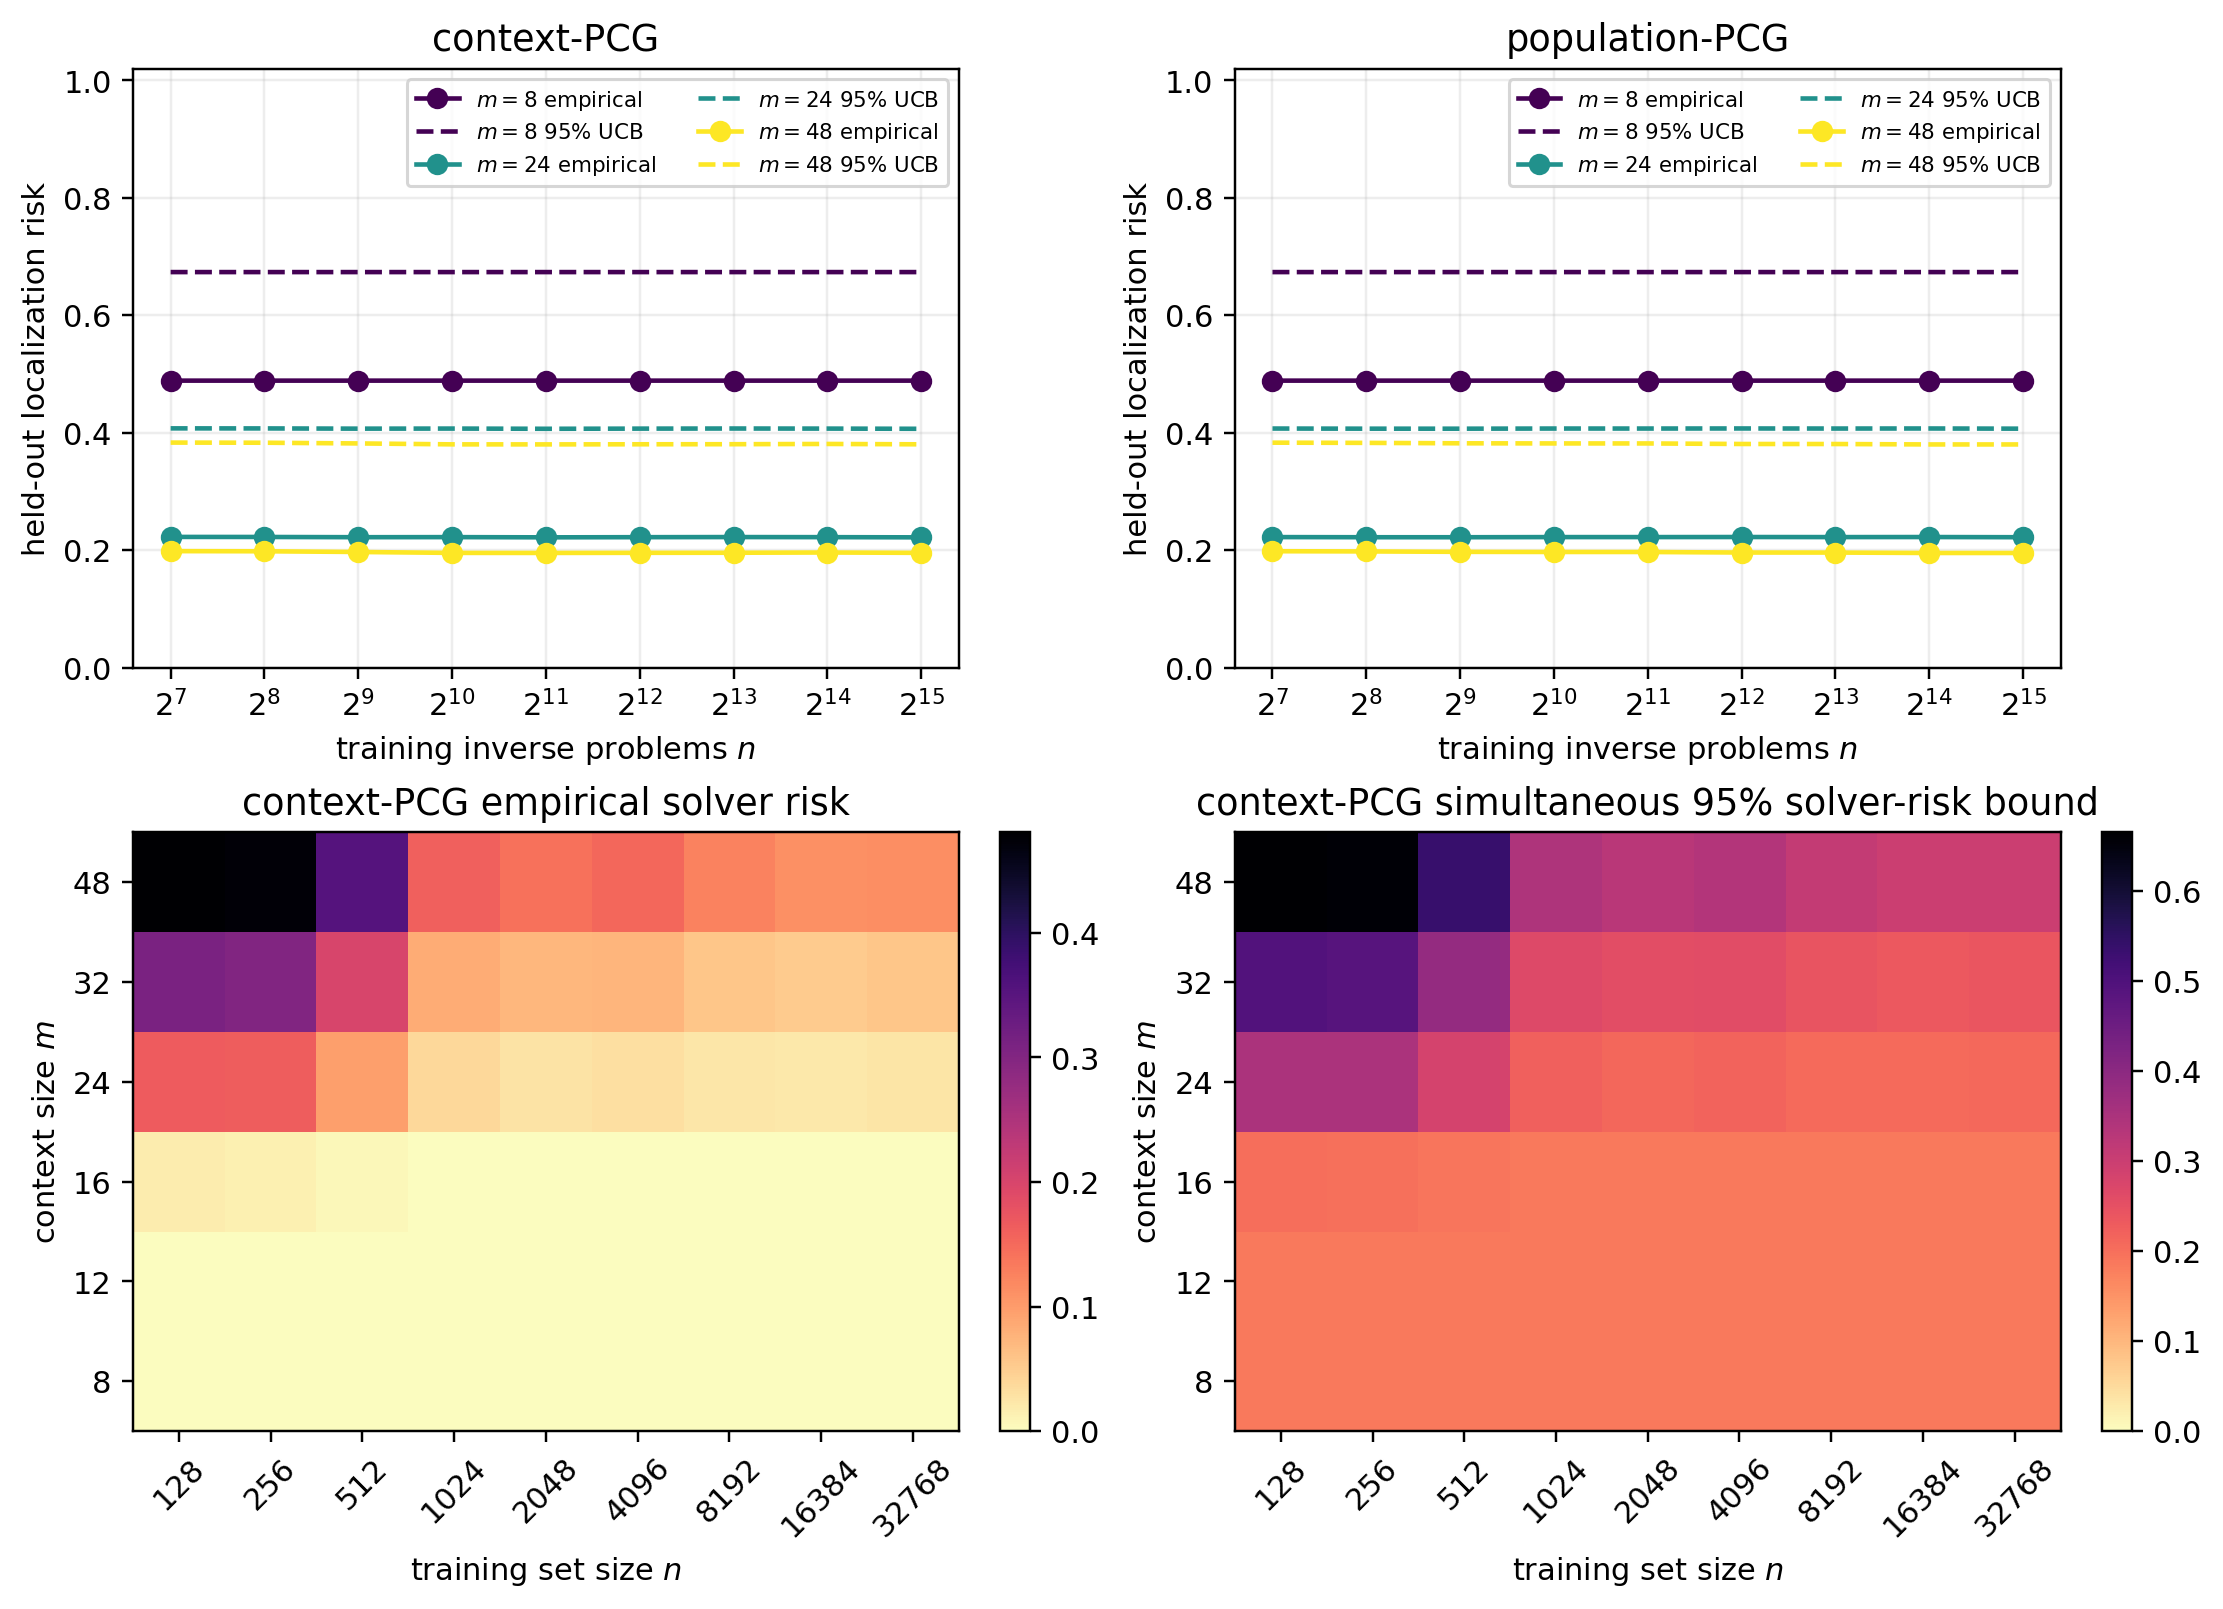
\includegraphics[width=0.98\linewidth]{scaling_generalization_bounds.png}
\caption{Empirical localization and numerical solver risks with simultaneous
95\% held-out upper bounds across dataset and context sizes.}
\label{fig:bounds}
\end{figure}


\begin{figure}[t]
\centering
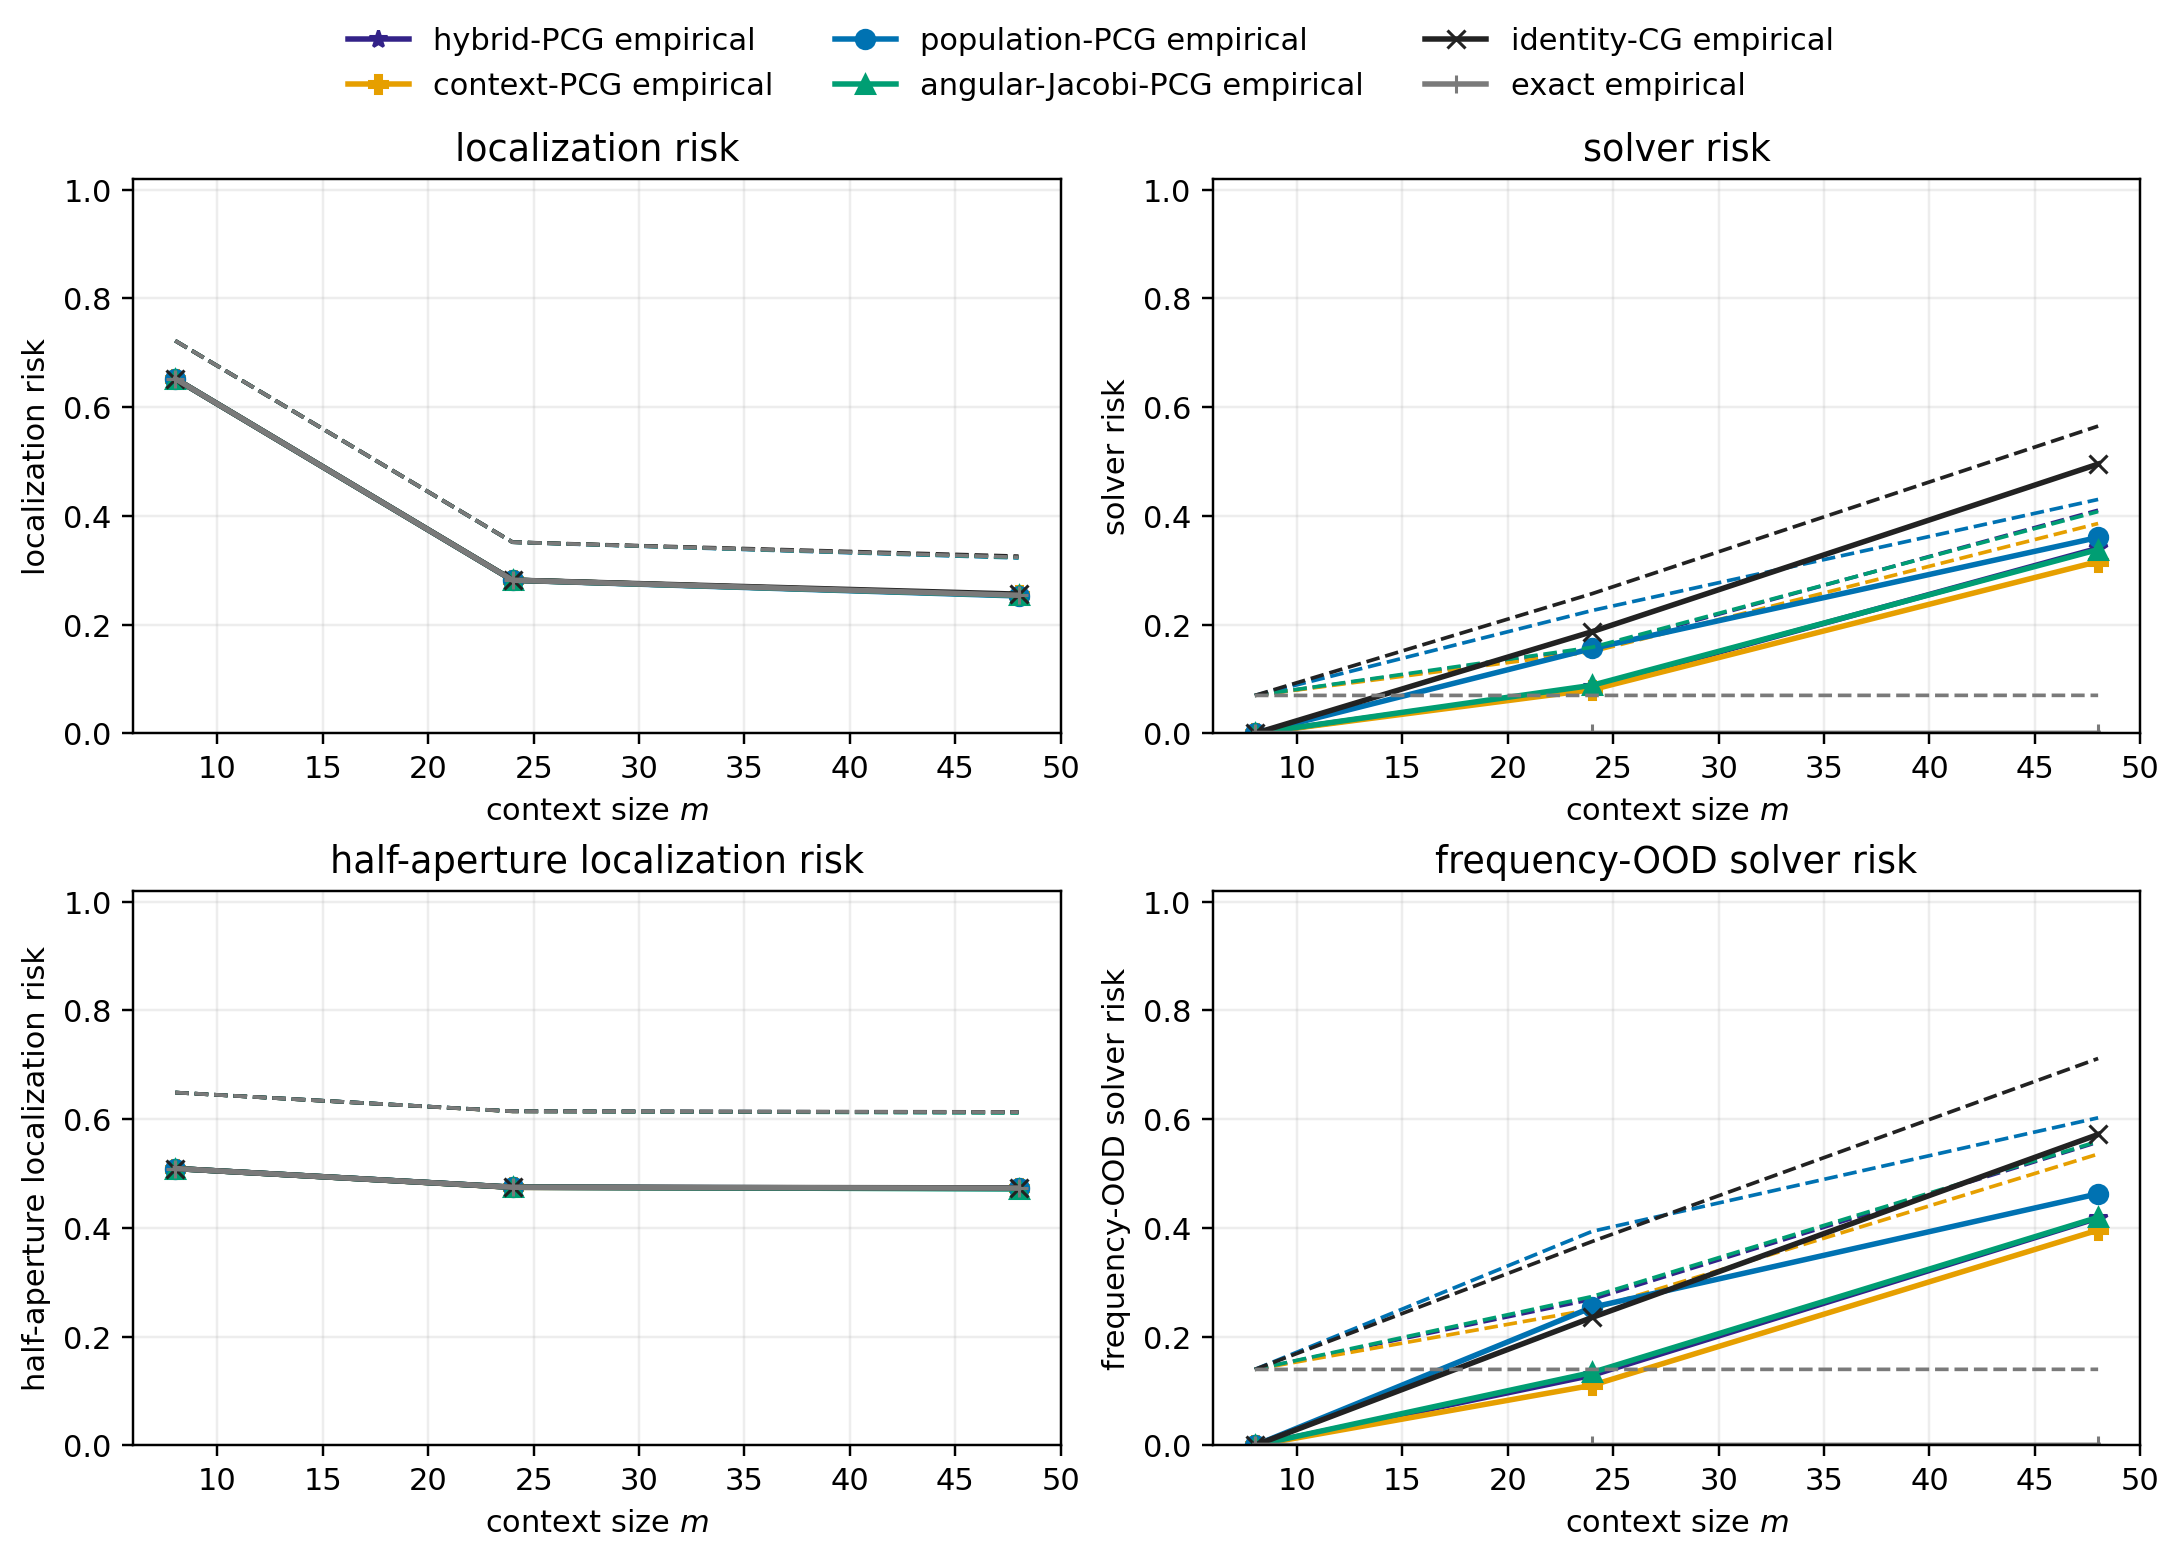
\includegraphics[width=0.98\linewidth]{scaling_geometry_generalization.png}
\caption{Independent-acquisition generalization.  Each bounded observation is
the mean of four fresh obstacle/noise tasks sharing one independently rotated
and jittered deterministic source--receiver geometry.  Dashed curves are
simultaneous 95\% Hoeffding upper bounds.}
\label{fig:geometry-bound}
\end{figure}


\FloatBarrier
\section{Results}
\begin{table}[t]
\centering\small
\caption{Final comparison at context $m=24$, width
128 and $n=32768$.  Baselines do
not train.  Runtime is milliseconds per held-out batch.}
\begin{tabular}{lcccccc}
\toprule Method & AP & $r_{\rm tr}$ mean & $r_{\rm tr}$ cov. & score error & 95\% cov. & ms\\
\midrule
hybrid-PCG & 0.774 & 0.030 & 4.16e-03 & 1.03e-03 & 0.970 & 8.372 \\
context-PCG & 0.774 & 0.028 & 4.09e-03 & 1.01e-03 & 0.968 & 8.338 \\
population-PCG & 0.774 & 0.065 & 7.41e-03 & 2.05e-03 & 0.943 & 7.548 \\
looped-HB & 0.505 & 0.127 & 0.020 & 0.104 & 0.167 & 20.629 \\
looped-Chebyshev & 0.651 & 0.093 & 0.028 & 0.125 & 0.225 & 17.850 \\
looped-Richardson & 0.300 & 0.259 & 0.074 & 0.256 & 0.045 & 17.597 \\
identity-CG & 0.774 & 0.222 & 7.29e-03 & 4.44e-03 & 0.955 & 7.289 \\
exact & 0.774 & 6.21e-05 & 1.67e-06 & 0 & 1.000 & 10.909 \\
\bottomrule
\end{tabular}
\end{table}

\begin{table}[t]
\centering\scriptsize
\caption{Scenario-wise comparison at the extrapolative context
$m=48$, width 128 and
$n=32768$.  Gains use the transformed-coordinate
residual $r_{\rm tr}$; values above one favor context-PCG.}
\begin{tabular}{lrrrrrr}
\toprule Scenario & AP CG & AP C-PCG & $r_{\rm tr}$ CG & $r_{\rm tr}$ C-PCG & mean gain & cov. gain\\
\midrule
ID four obstacles & 0.809 & 0.812 & 0.963 & 0.129 & 7.460 & 2.939 \\
ID one obstacle & 0.987 & 0.988 & 2.070 & 0.140 & 14.820 & 1.489 \\
OOD 30 percent noise & 0.781 & 0.782 & 0.415 & 0.045 & 9.126 & 4.776 \\
OOD half aperture & 0.546 & 0.545 & 0.966 & 0.234 & 4.126 & 1.280 \\
OOD six obstacles & 0.775 & 0.776 & 0.843 & 0.103 & 8.180 & 4.402 \\
OOD stars & 0.812 & 0.821 & 0.859 & 0.114 & 7.534 & 2.366 \\
OOD wavenumber 12 & 0.856 & 0.861 & 1.311 & 0.194 & 6.773 & 2.362 \\
\bottomrule
\end{tabular}
\end{table}

On the original scaling grid, prompt-conditioned PCG lowers the
transformed-coordinate posterior-mean residual relative to CG in
7 of
7 held-out scenarios at $m=
48$.  Its worst scenario-wise gain is
4.126$\times$
and its median gain is
7.534$\times$.
All 21 individual
training-seed/scenario cells favor context-PCG; the smallest such gain is
3.507$\times$.
The largest absolute AP change is only
8.20e-03; hence
the learned conditioner is substantially more accurate in score fidelity while
localization effectiveness remains essentially tied at the physical
point-spread limit.
At $m=48$, context-PCG attains numerical 95\% band
coverage 0.865,
compared with 0.244
for CG.  This is UQ fidelity to the exact Bayesian solve, not a physical
coverage claim.
The foundation-model width sweep also rejects a ``bigger is automatically
better'' interpretation.  Width 64 gives the
smallest extrapolative transformed residual, while width
512 has
22.451$\times$
as many parameters and a
1.035$\times$
larger residual.  The controller has reached a feature/basis plateau rather
than a parameter-limited regime.


\begin{figure}[t]
\centering
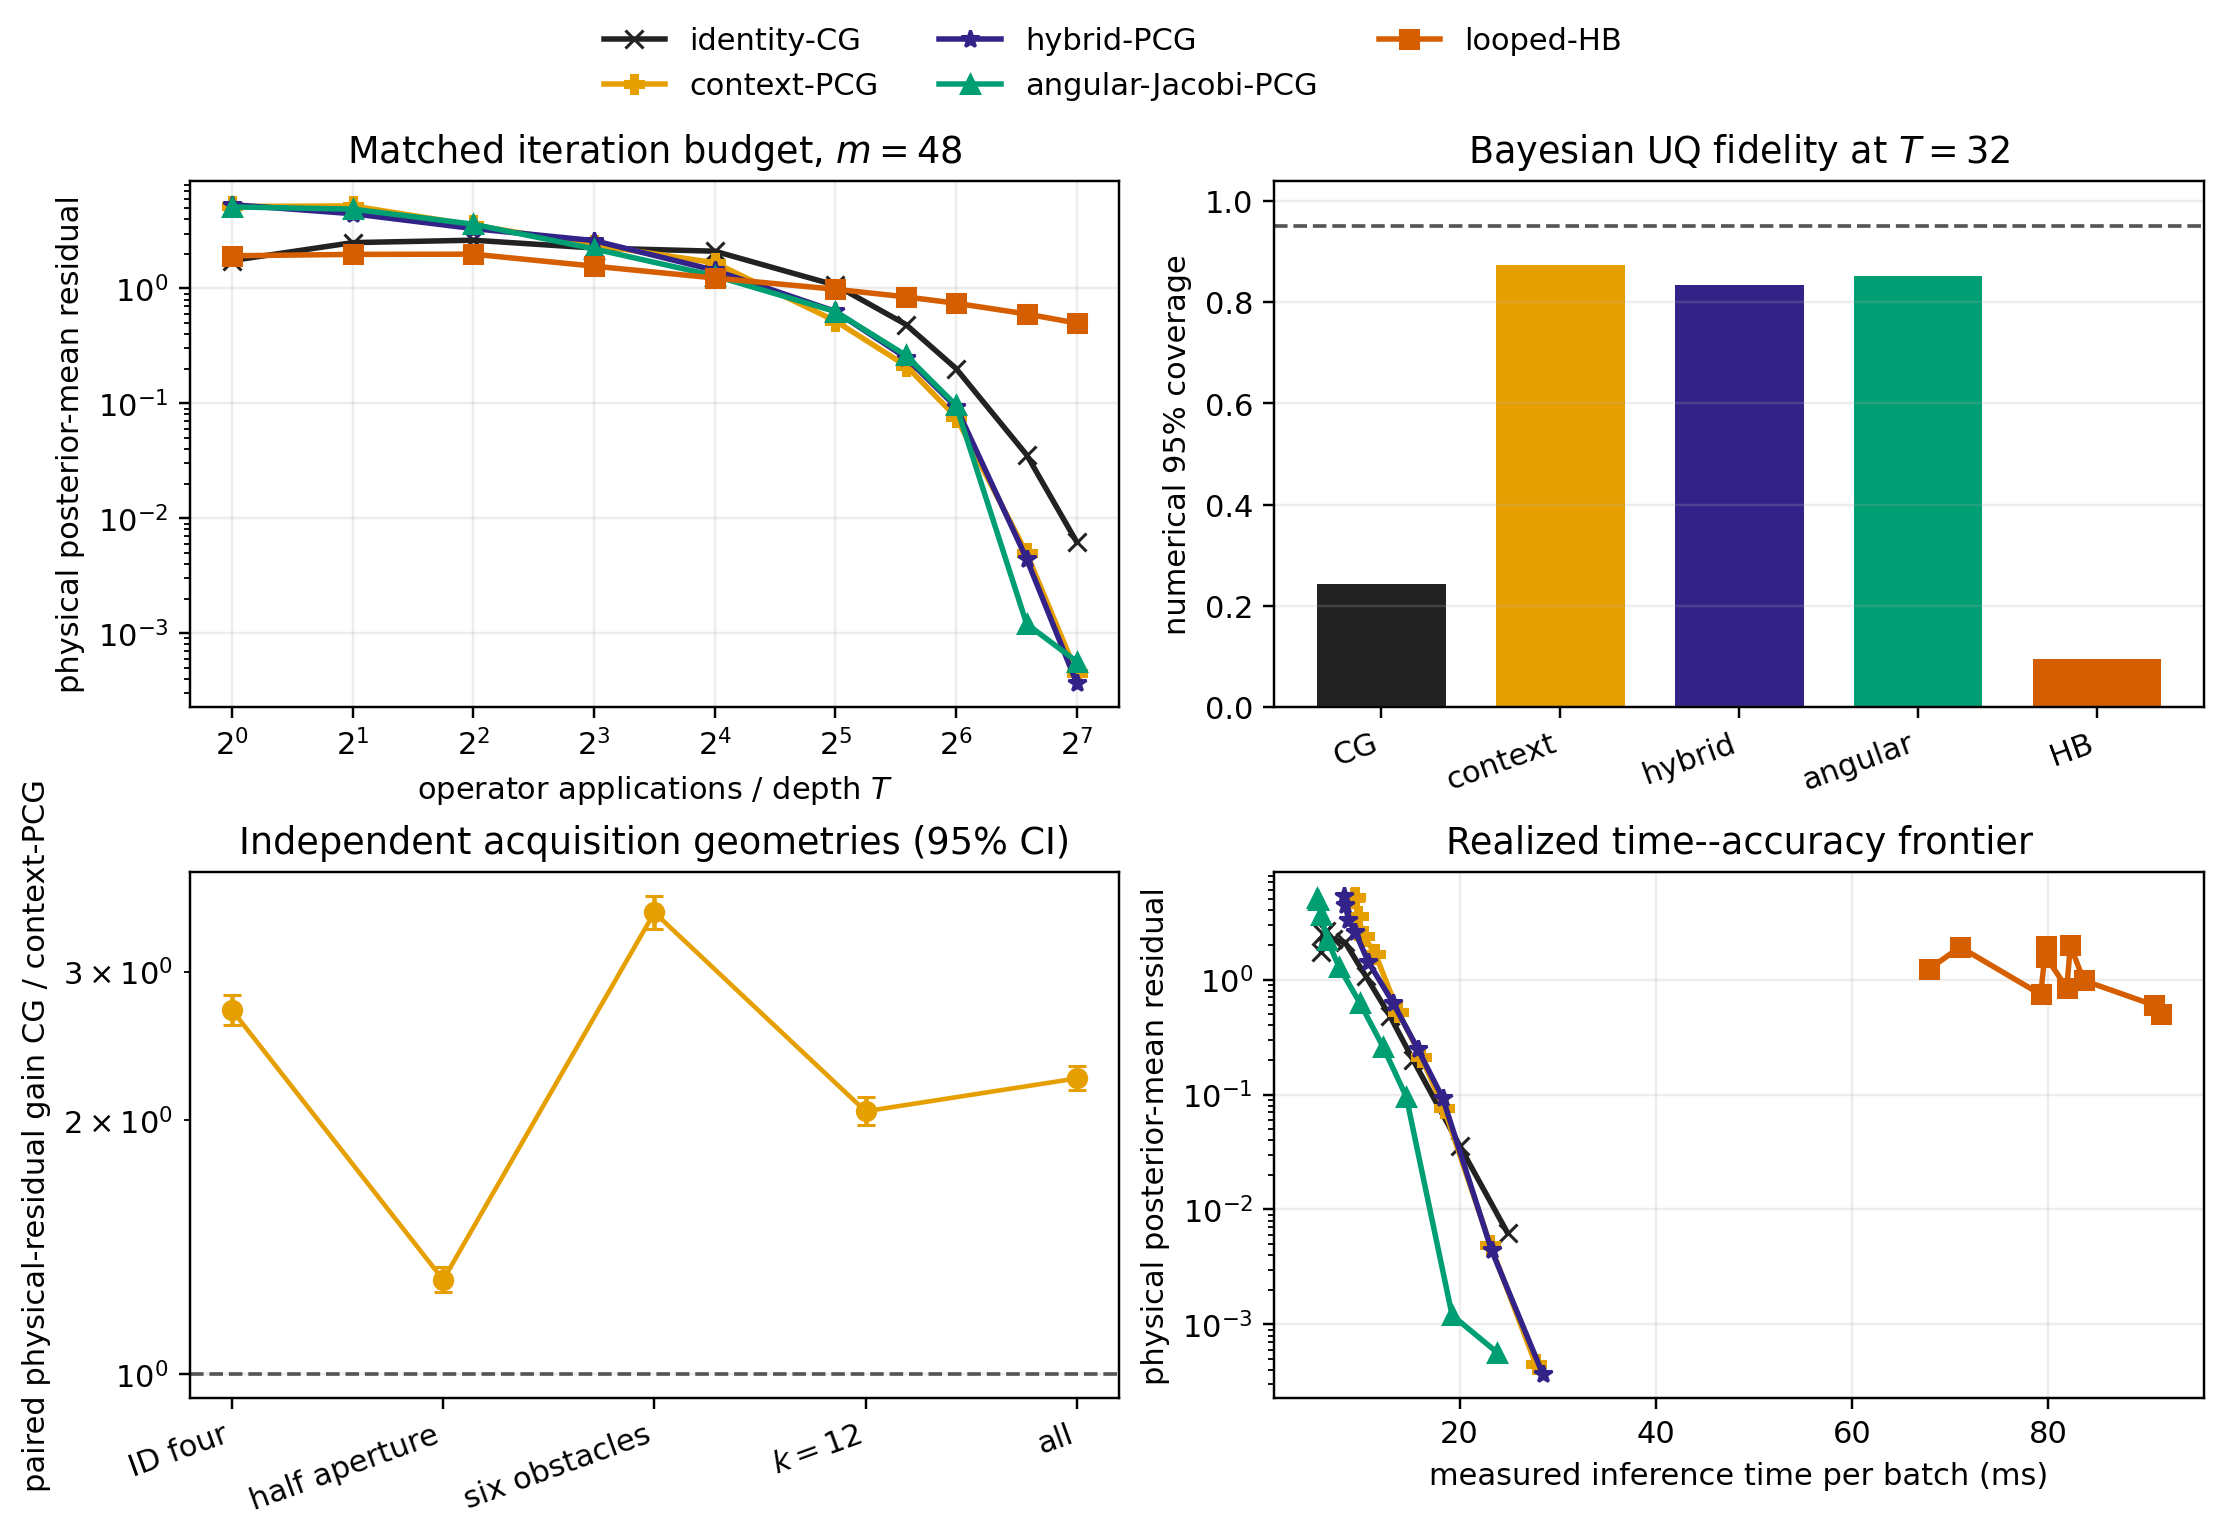
\includegraphics[width=0.98\linewidth]{scaling_cg_comparison.png}
\caption{Direct comparison with ordinary CG.  Top left: matched operator
applications.  Top right: numerical Bayesian coverage relative to the exact
solve.  Bottom left: paired physical-residual gains on independent acquisition
geometries.  Bottom right: measured time--accuracy paths.  Values above one in
the gain panel favor context-PCG.}
\label{fig:cg-comparison}
\end{figure}



\begin{figure}[t]
\centering
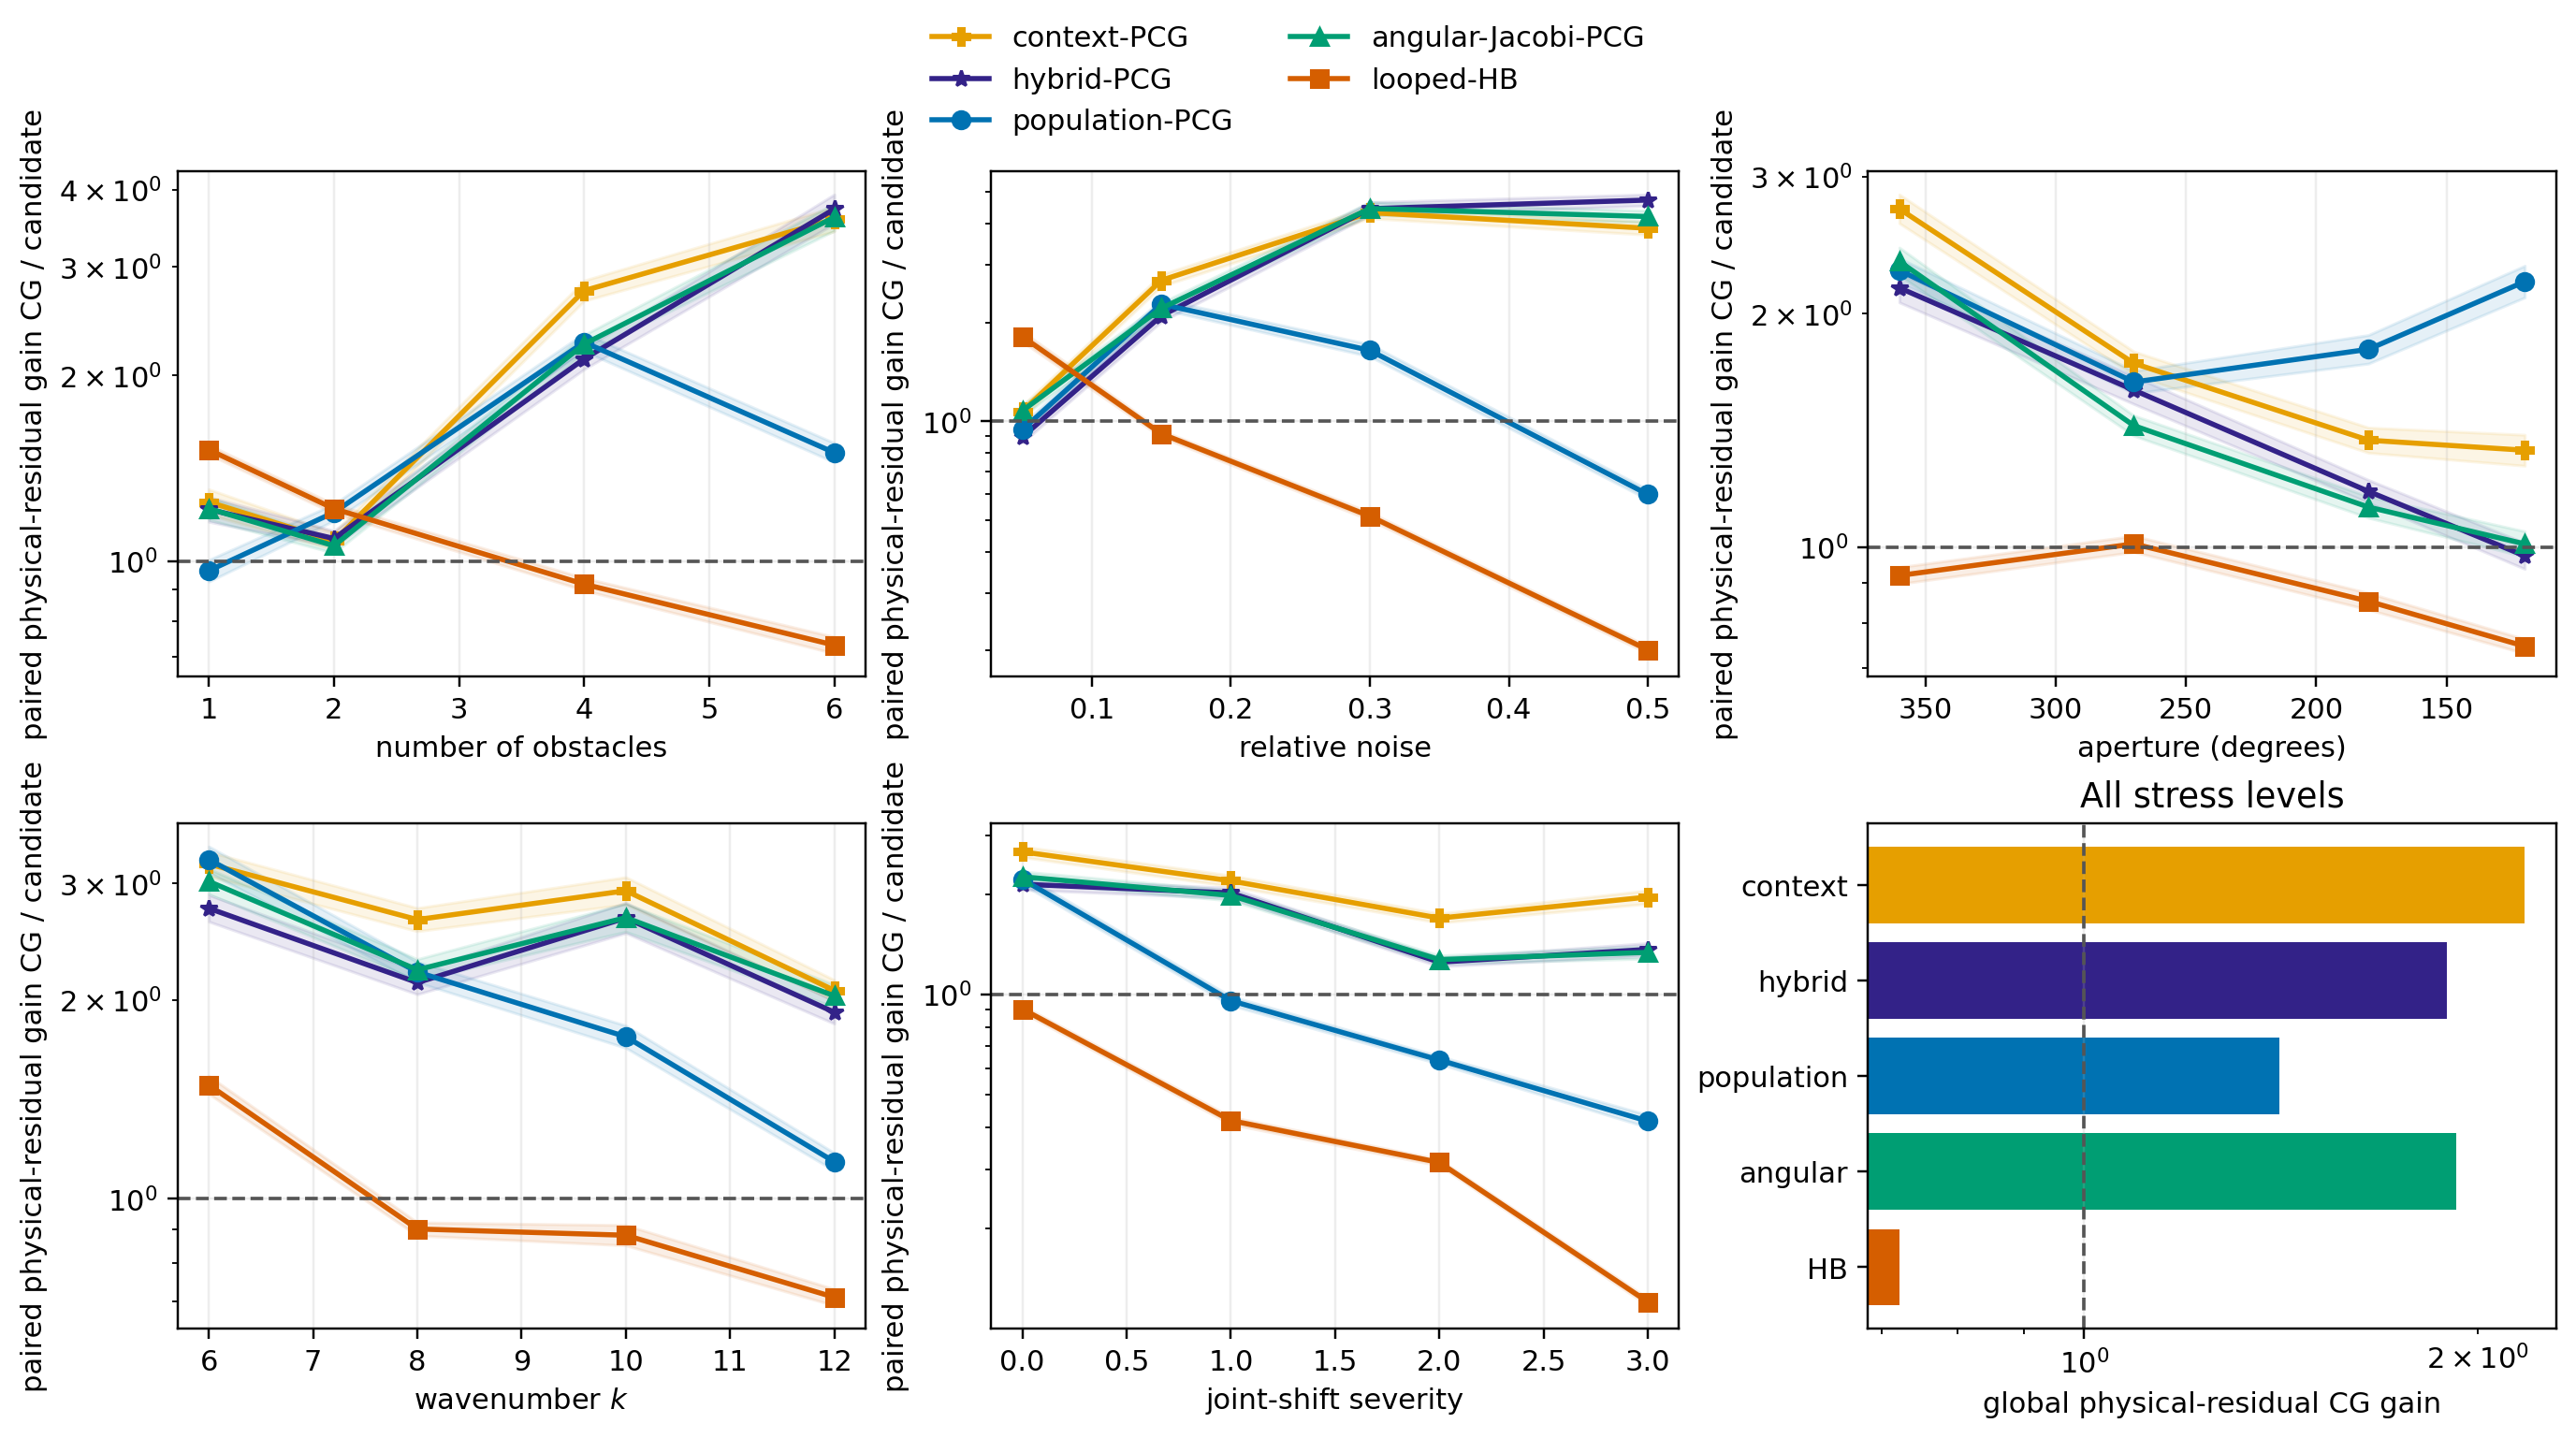
\includegraphics[width=0.98\linewidth]{scaling_cg_stress_test.png}
\caption{Marginal and joint physical stress sweeps at
$m=48$ and $T=32$.  Curves are paired geometric-mean
physical-coordinate residual gains over at least
192 independent acquisition
batches per level; shaded regions are pointwise 95\% normal-approximation
log-ratio intervals.  Values above
one favor the preconditioned method over ordinary CG.}
\label{fig:cg-stress}
\end{figure}

Across the 20 stress levels, the
context-PCG gain over CG ranges from
1.071$\times$ to
4.321$\times$; its
smallest paired-batch win rate at any level is
0.625.  The first
sixteen levels vary one factor; the four joint-severity levels co-vary obstacle
count, noise, aperture, frequency and acquisition jitter.  These remain
simulator perturbations, not a certificate for arbitrary distribution shift.
Context-PCG has the smallest residual in
11 of the
20 levels, versus
1 for angular-Jacobi,
3 for population-PCG and
2 for the hybrid, while looped HB
wins 3.  Robustly beating CG therefore
does not imply dominance over every informed preconditioner.
Across all stress batches, context-PCG's geometric-mean residual gain is
2.172$\times$, with
AP and numerical-coverage changes
1.08e-03 and
0.539 relative
to CG.  Looped HB attains a residual gain of
0.723$\times$ but changes
AP by -0.300 and coverage by
-0.257.  Its occasional
short-horizon residual win is therefore not a reconstruction or UQ win.
At the most extreme joint shift, context-PCG retains a residual gain of
1.958$\times$
(95\% interval
[1.870,
2.050]) and
wins 0.974 of
paired batches (Wilson 95\% interval
[0.940,
0.989]).
Angular-Jacobi retains
1.337$\times$, whereas
population-PCG and looped HB fall to
0.418$\times$ and
0.120$\times$.  The
context-PCG coverage gain is nevertheless
0:
this is residual robustness, not universal UQ calibration.



\begin{figure}[t]
\centering
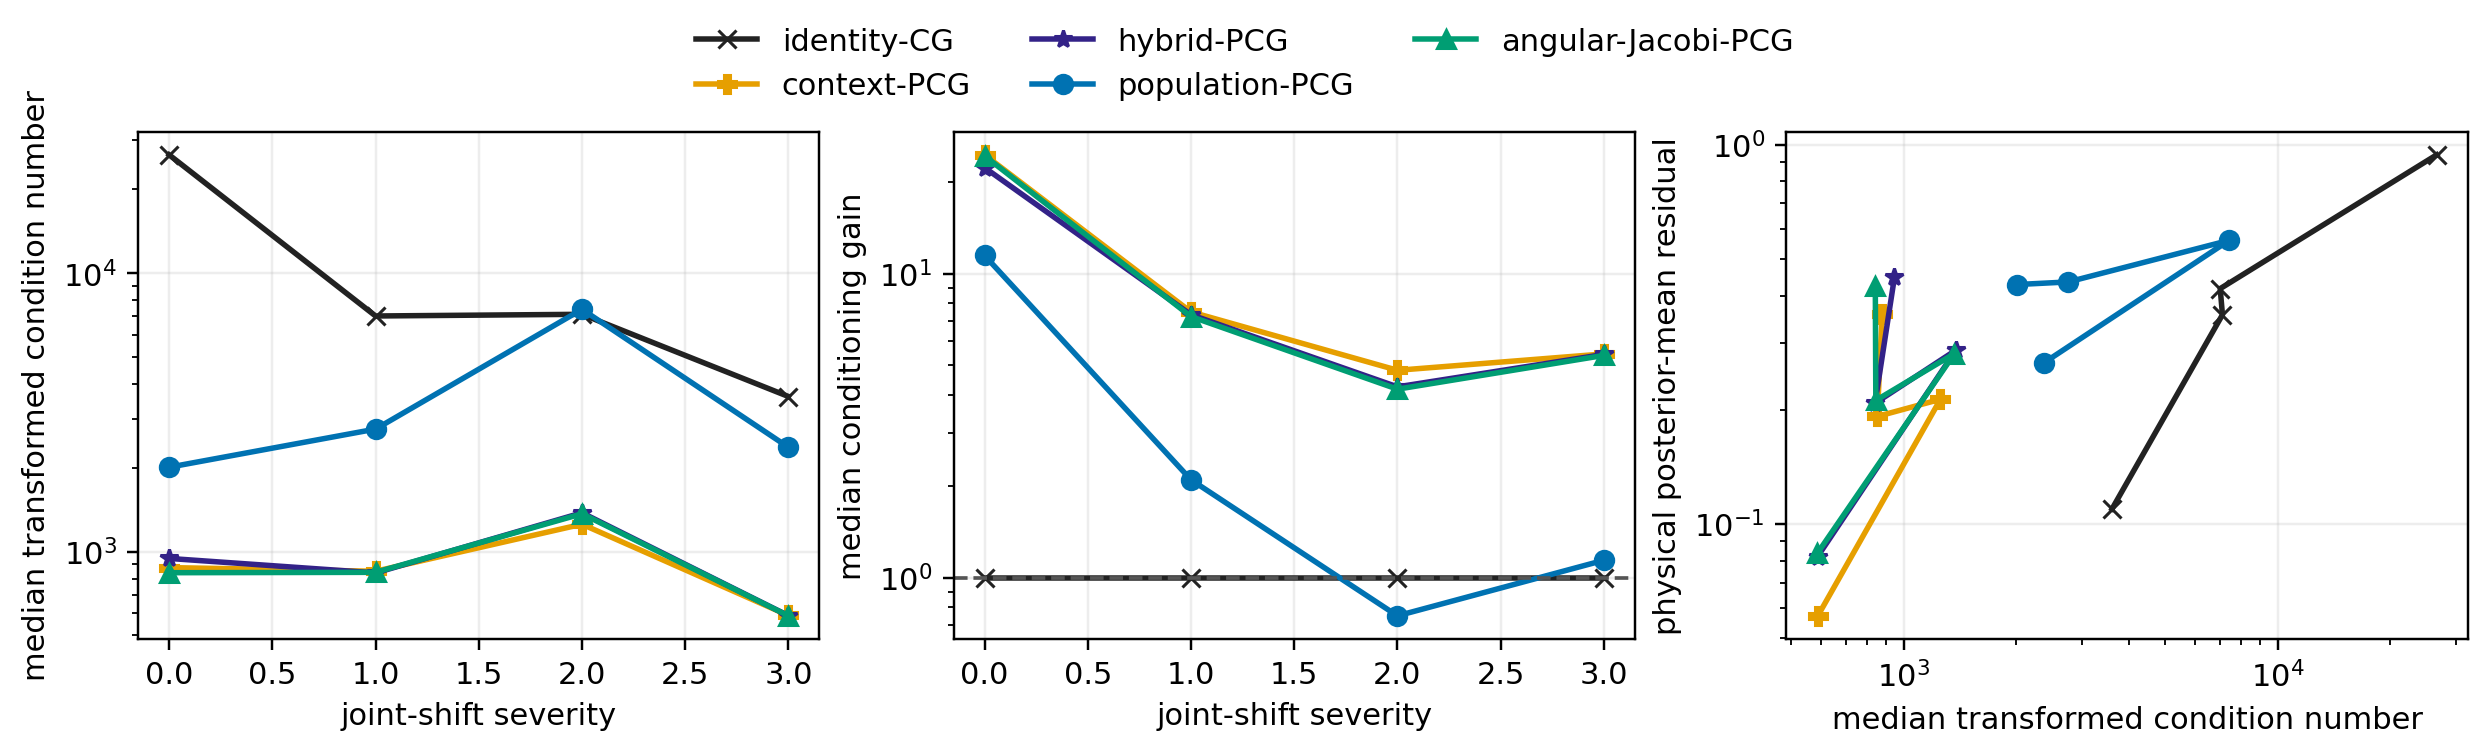
\includegraphics[width=0.98\linewidth]{scaling_joint_conditioning.png}
\caption{Spectral mechanism across the four joint-shift severities.  Each
point aggregates independent acquisition batches; the right panel links
condition compression to the observed finite-depth physical residual.}
\label{fig:joint-conditioning}
\end{figure}

At the extreme joint shift, the raw median condition number is
3.61e+03.  Context-PCG
reduces it by
5.448$\times$
to 589.921, whereas
angular-Jacobi reduces it by
5.387$\times$
to 588.200.  The
commutator is 0.329.
Context and angular-Jacobi therefore have nearly identical scalar condition
numbers but residual gains
1.958$\times$ and
1.337$\times$.
Condition number alone does not rank the finite-horizon solve; spectral
clustering and right-hand-side alignment matter, while the nonzero commutator
still limits both fixed-basis factors.



\begin{figure}[p]
\centering
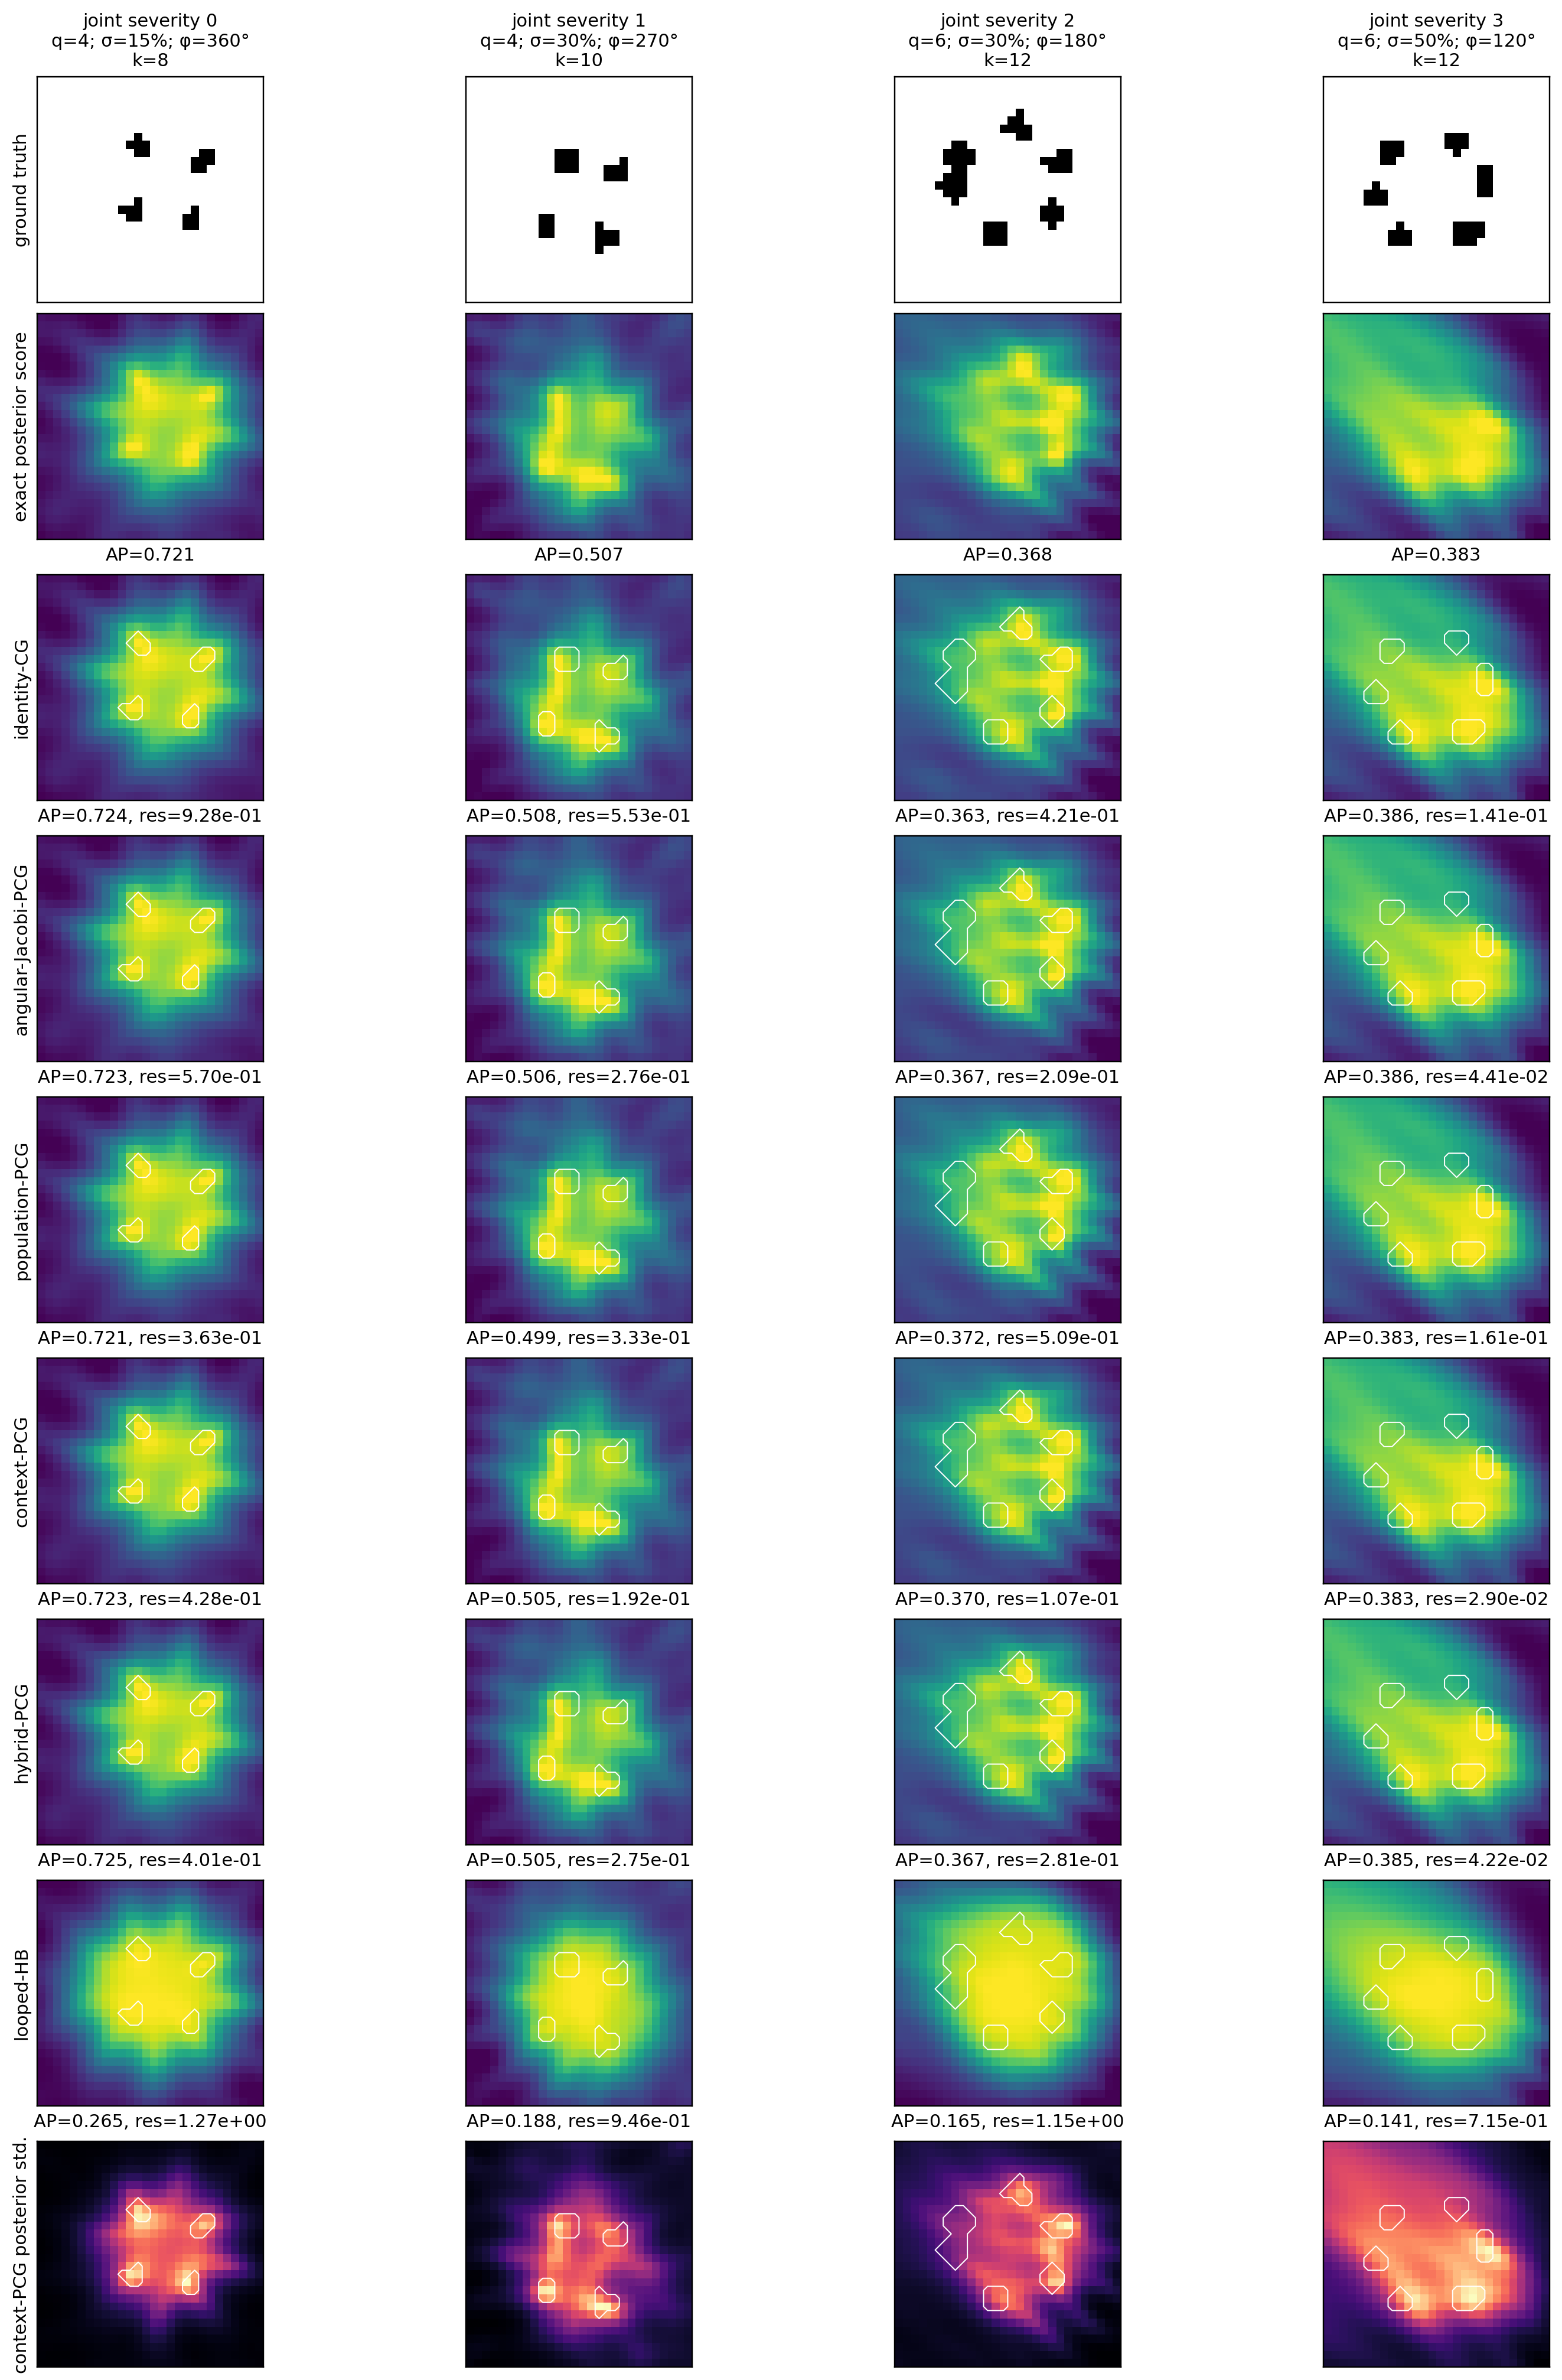
\includegraphics[width=0.94\linewidth,height=0.88\textheight,keepaspectratio]{scaling_joint_reconstructions.png}
\caption{Pre-specified reconstructions along the joint-shift path (seed 17,
geometry draw zero, task zero); no task was selected by performance.  White
contours show the true obstacles.  Each score map is normalized by its own
1st--99th percentile range to compare localization shape; AP and physical
residual are reported separately.  Context-PCG preserves the exact LSM ranking
while lowering the finite-depth residual, whereas looped HB has poor ranking
despite some residual improvement.  The last row is context-PCG posterior
standard deviation, not a reconstruction score.}
\label{fig:joint-reconstructions}
\end{figure}



The equal-budget transformed-coordinate residual ratios at the final central
configuration are
3.407$\times$ for
the posterior mean and
0.985$\times$
for posterior covariance.  Ratios above one mean that the learned factor lowers
the transformed-coordinate optimization metric.  Since the coordinate factor
differs by method, these ratios are not interpreted as physical solver gains;
the common-coordinate audit below supplies that comparison.  Localization can
nevertheless saturate before residual convergence; in that regime additional
solver accuracy does not overcome the physical point-spread limit.
Across all six contexts, the corresponding gains are
4.336$\times$
and
1.535$\times$.
At the extrapolative context $m=48$ they reach
4.703$\times$
and
1.909$\times$,
respectively.  Thus the transformed training-metric separation grows with
context, although covariance separation is not uniform.  Whether this survives
in the physical coordinate is evaluated separately below.


At the same central configuration, prompt-conditioned PCG improves ordinary
CG in transformed-coordinate residual by
8.030$\times$
on the posterior mean and
1.785$\times$
on posterior covariance.  Across all contexts its corresponding gains are
7.936$\times$
and
2.183$\times$.
This is a diagnostic of whether the current operator carries useful in-context
signal within the prescribed optimization coordinates; it is not the direct
physical CG claim.  The post-training $r_{\rm phys}$ audit below provides the
coordinate-invariant test.
Within the shared model implementation, the price is controller overhead:
context-PCG costs
1.144$\times$ the
CG batch time at $m=24$ and
1.269$\times$ at
$m=48$.  It is therefore iteration-efficient, not a
large wall-clock speedup at fixed depth.  After removing the unused endpoint
controller from PCG inference, the iterative methods are faster than dense
factorization on the tested batches.  The optimized classical controls below
provide the stricter timing comparison.



We also test an analytic--learned hybrid: the current Hessian is rotated into
the prescribed GP angular feature basis, its diagonal supplies a training-free
positive preconditioner, and a zero-initialized context network learns only a
multiplicative residual correction.  At the central configuration it improves
CG in transformed-coordinate residual by
7.500$\times$
for the mean and
1.751$\times$
for covariance.  Across all contexts the corresponding gains are
6.116$\times$
and
2.041$\times$.
At $m=48$ and $T=32$, however, its physical mean residual is
0.630,
whereas context-PCG attains
0.521
and analytic angular-Jacobi attains
0.629.
The angular-to-hybrid residual ratio is
0.997;
at the common central width this tests whether the correction improves the
analytic base without extra capacity.  Across the width sweep, the best hybrid
uses width 64 and attains transformed residual
0.178, covariance
residual
0.014, and
coverage 0.837.
These width-sweep residuals are in transformed coordinates and are therefore
not divided by the physical residual of the analytic control; their homogeneous
physical comparison is the matched-width, matched-depth audit above.
This control is the criterion for deciding whether preconditioning needs to be
learned rather than merely computed in context.



The post-training depth audit contains
71,568 task-level evaluations over
$T\in[1, 2, 4, 8, 16, 32, 48, 64, 96, 128]$.  At the extrapolative context
$m=48$, the CG-to-population-PCG physical
posterior-mean residual gain is
1.585$\times$
at $T=32$ and
2.119$\times$
at $T=64$; the corresponding prompt-conditioned gains are
2.049$\times$
and
2.641$\times$.
At the same two depths, context-PCG improves looped HB by
1.887$\times$ and
9.771$\times$,
respectively; HB has a competitive short-horizon transient but its stationary
recurrence does not retain the long-depth Krylov convergence.
At $m=48$ and $T=32$, looped HB has mean residual
0.983,
average precision
0.478,
and numerical 95\% coverage
0.095; its
batch runtime is
83.616 ms.
Its relative LSM-score error is
0.139,
versus 0.029
for CG and
4.54e-03
for context-PCG.  In an ill-conditioned system, a smaller Euclidean residual
can still leave larger solution error along small-eigenvalue directions; this
explains why HB's residual transient does not produce a good reconstruction.
Thus its residual improvement over CG does not translate into faithful LSM
localization or calibrated Bayesian uncertainty, and its dense learned update
is substantially more expensive than Krylov PCG.
At $T=128$, the equal-depth CG-to-context-PCG gain reaches
13.847$\times$;
this ratio is taken near the numerical convergence floor and is not a claim of
improved physical localization.
For a tolerance-oriented comparison at $m=48$,
context-PCG first reaches mean residual $0.1$ at $T=
64$, versus $T=
96$ for CG; for residual $0.01$ the
depths are 96 and
128.
At the $0.01$ target, however, the measured batch times are
23.128 ms and
24.912 ms, respectively:
the optimized implementation preserves a modest wall-clock benefit from the
iteration-count saving at this matrix size.
Figure~\ref{fig:depth} therefore distinguishes a genuine
conditioning advantage from merely granting the learned method more
iterations.  The fact that depth remains useful at large $m$ is qualitatively
consistent with the randomly rotated structured-covariance regime of
Bordelon et al.; it is not an assertion that their linear-model asymptotics
govern this inverse-scattering system.



At $m=48$, the median condition-number reduction is
10.473$\times$
for population-PCG and
23.220$\times$
for context-PCG.  Figure~\ref{fig:conditioning} directly checks whether
smaller residuals track spectral compression and whether the obstacle-dependent
operator commutes with the fixed GP geometry.
The analytic--learned hybrid reduces the condition number by
20.328$\times$
and leaves median condition number
1.25e+03.
The raw median condition number is still
2.66e+04, and
context-PCG leaves
1.09e+03; the
normalized commutator
0.221
therefore identifies the remaining inability of fixed modal gains to rotate
task-dependent eigendirections.



The training-free angular-Jacobi control is the critical test of whether the
available in-context signal actually needs to be learned.  At
$m=48$ and $T=32$, its physical posterior-mean residual is
0.629, versus
0.521
for context-PCG, a classical-to-learned ratio of
1.207.
At $T=96$ the ratio is instead
0.243,
so the analytical control overtakes the learned finite-horizon factor at high
accuracy.
Their numerical 95\% band coverages at $T=32$ are
0.851 and
0.873, respectively.
Its transformed condition number is
1.01e+03 and its runtime
is 9.836 ms, or
0.715$\times$
the learned method.  Removing unused feature/controller calculations from CG
also reduces its $T=32$ runtime to
8.809 ms; context-PCG
is then
1.561$\times$
slower.  At residual target $0.01$, angular-Jacobi reaches the target at
$T=96$ in
19.240 ms;
optimized CG uses $T=
128$ and
22.862
ms, while context-PCG uses
23.128 ms.
Across all 18 context/target cells in
Figure~\ref{fig:tolerance-frontier}, angular-Jacobi is fastest in
11, hybrid-PCG in
0, population-PCG in
0, identity-CG in
0, optimized CG in
5, block-Jacobi in
2 and context-PCG in
0.  Hence context-PCG's equal-depth
advantage does not become a strict wall-clock win against every optimized
operator-aware baseline.
Thus the experiment supports learning the conditioner
only to the extent that it improves or amortizes this cheap operator-aware
baseline; diagonal and local block-Jacobi in the physical ordering do not
extract the same angular GP structure.


The fitted powers must also be read diagnostically rather than as universal
laws.  For population-PCG the localization fit has $R^2=
0.984$, whereas the
solver-risk fit has $R^2=
0.775$.  A low or negative
$R^2$ rejects the proposed monotone separable power-law description on this
finite grid; it is evidence of non-monotone optimization or a performance
plateau, not a scaling exponent to extrapolate.  Exponents reported as 3.000
hit the fit's upper constraint and must be read as boundary estimates, not
identified power laws.


\FloatBarrier
\begin{figure}[t]
\centering
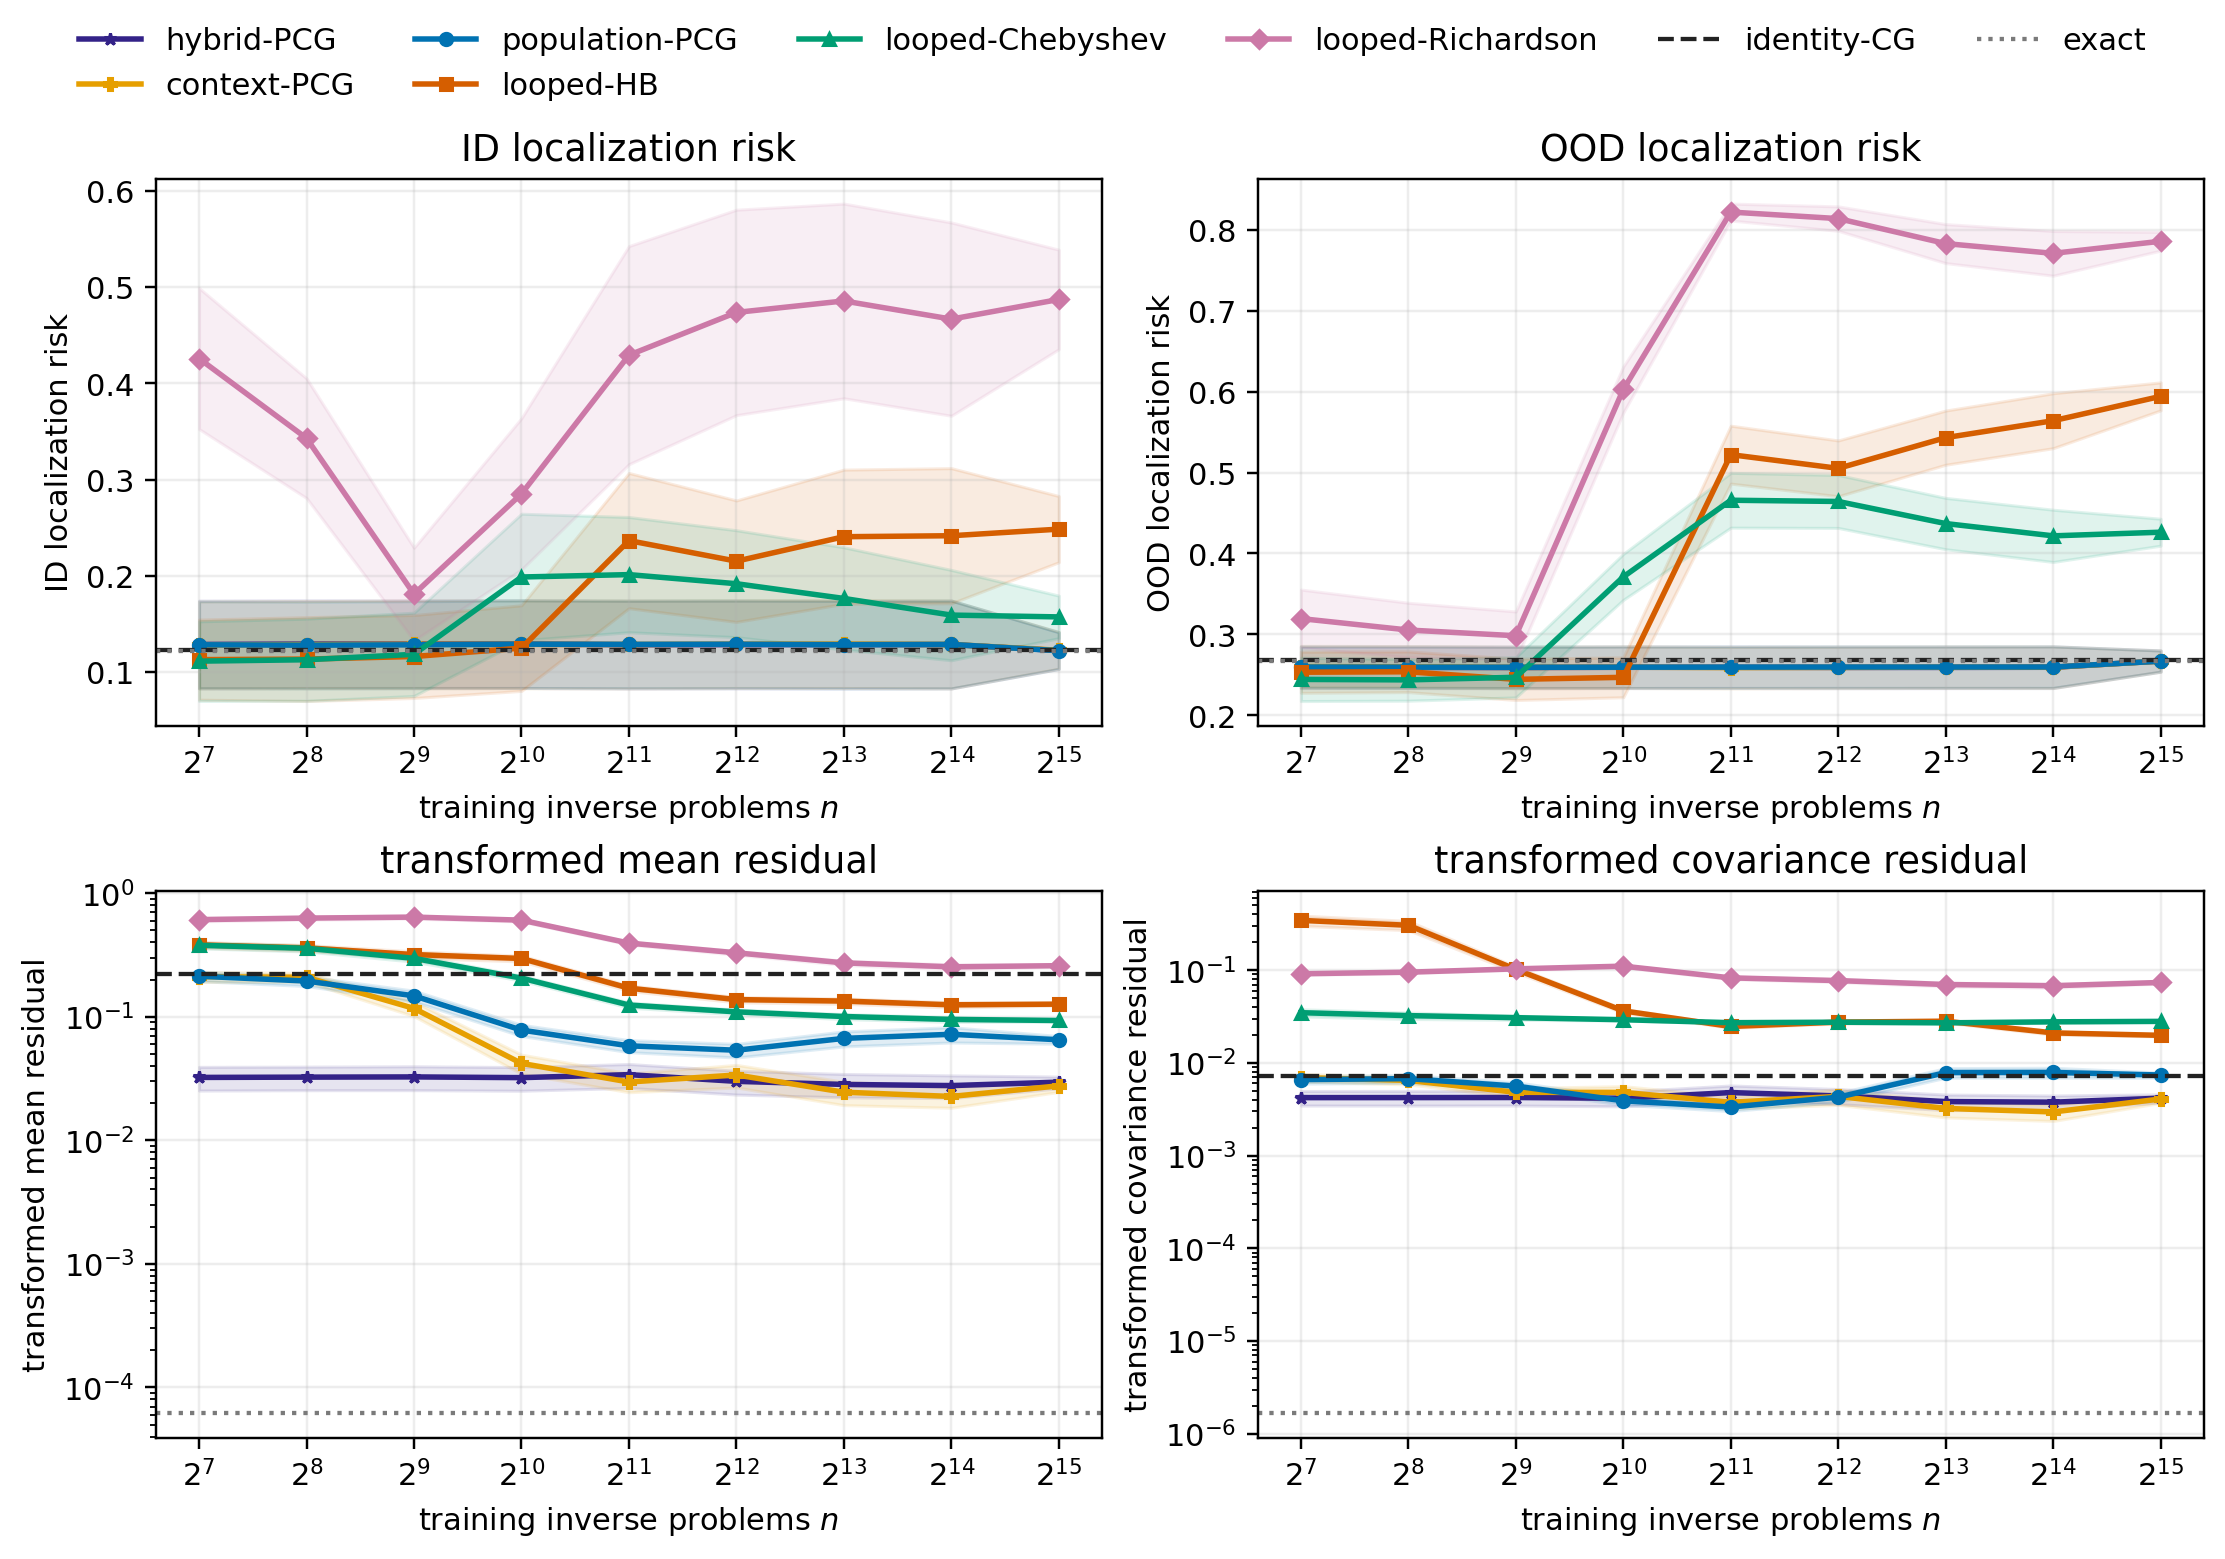
\includegraphics[width=0.98\linewidth]{scaling_dataset.png}
\caption{Learning curves in dataset size at fixed network width and context.}
\end{figure}

\begin{figure}[t]
\centering
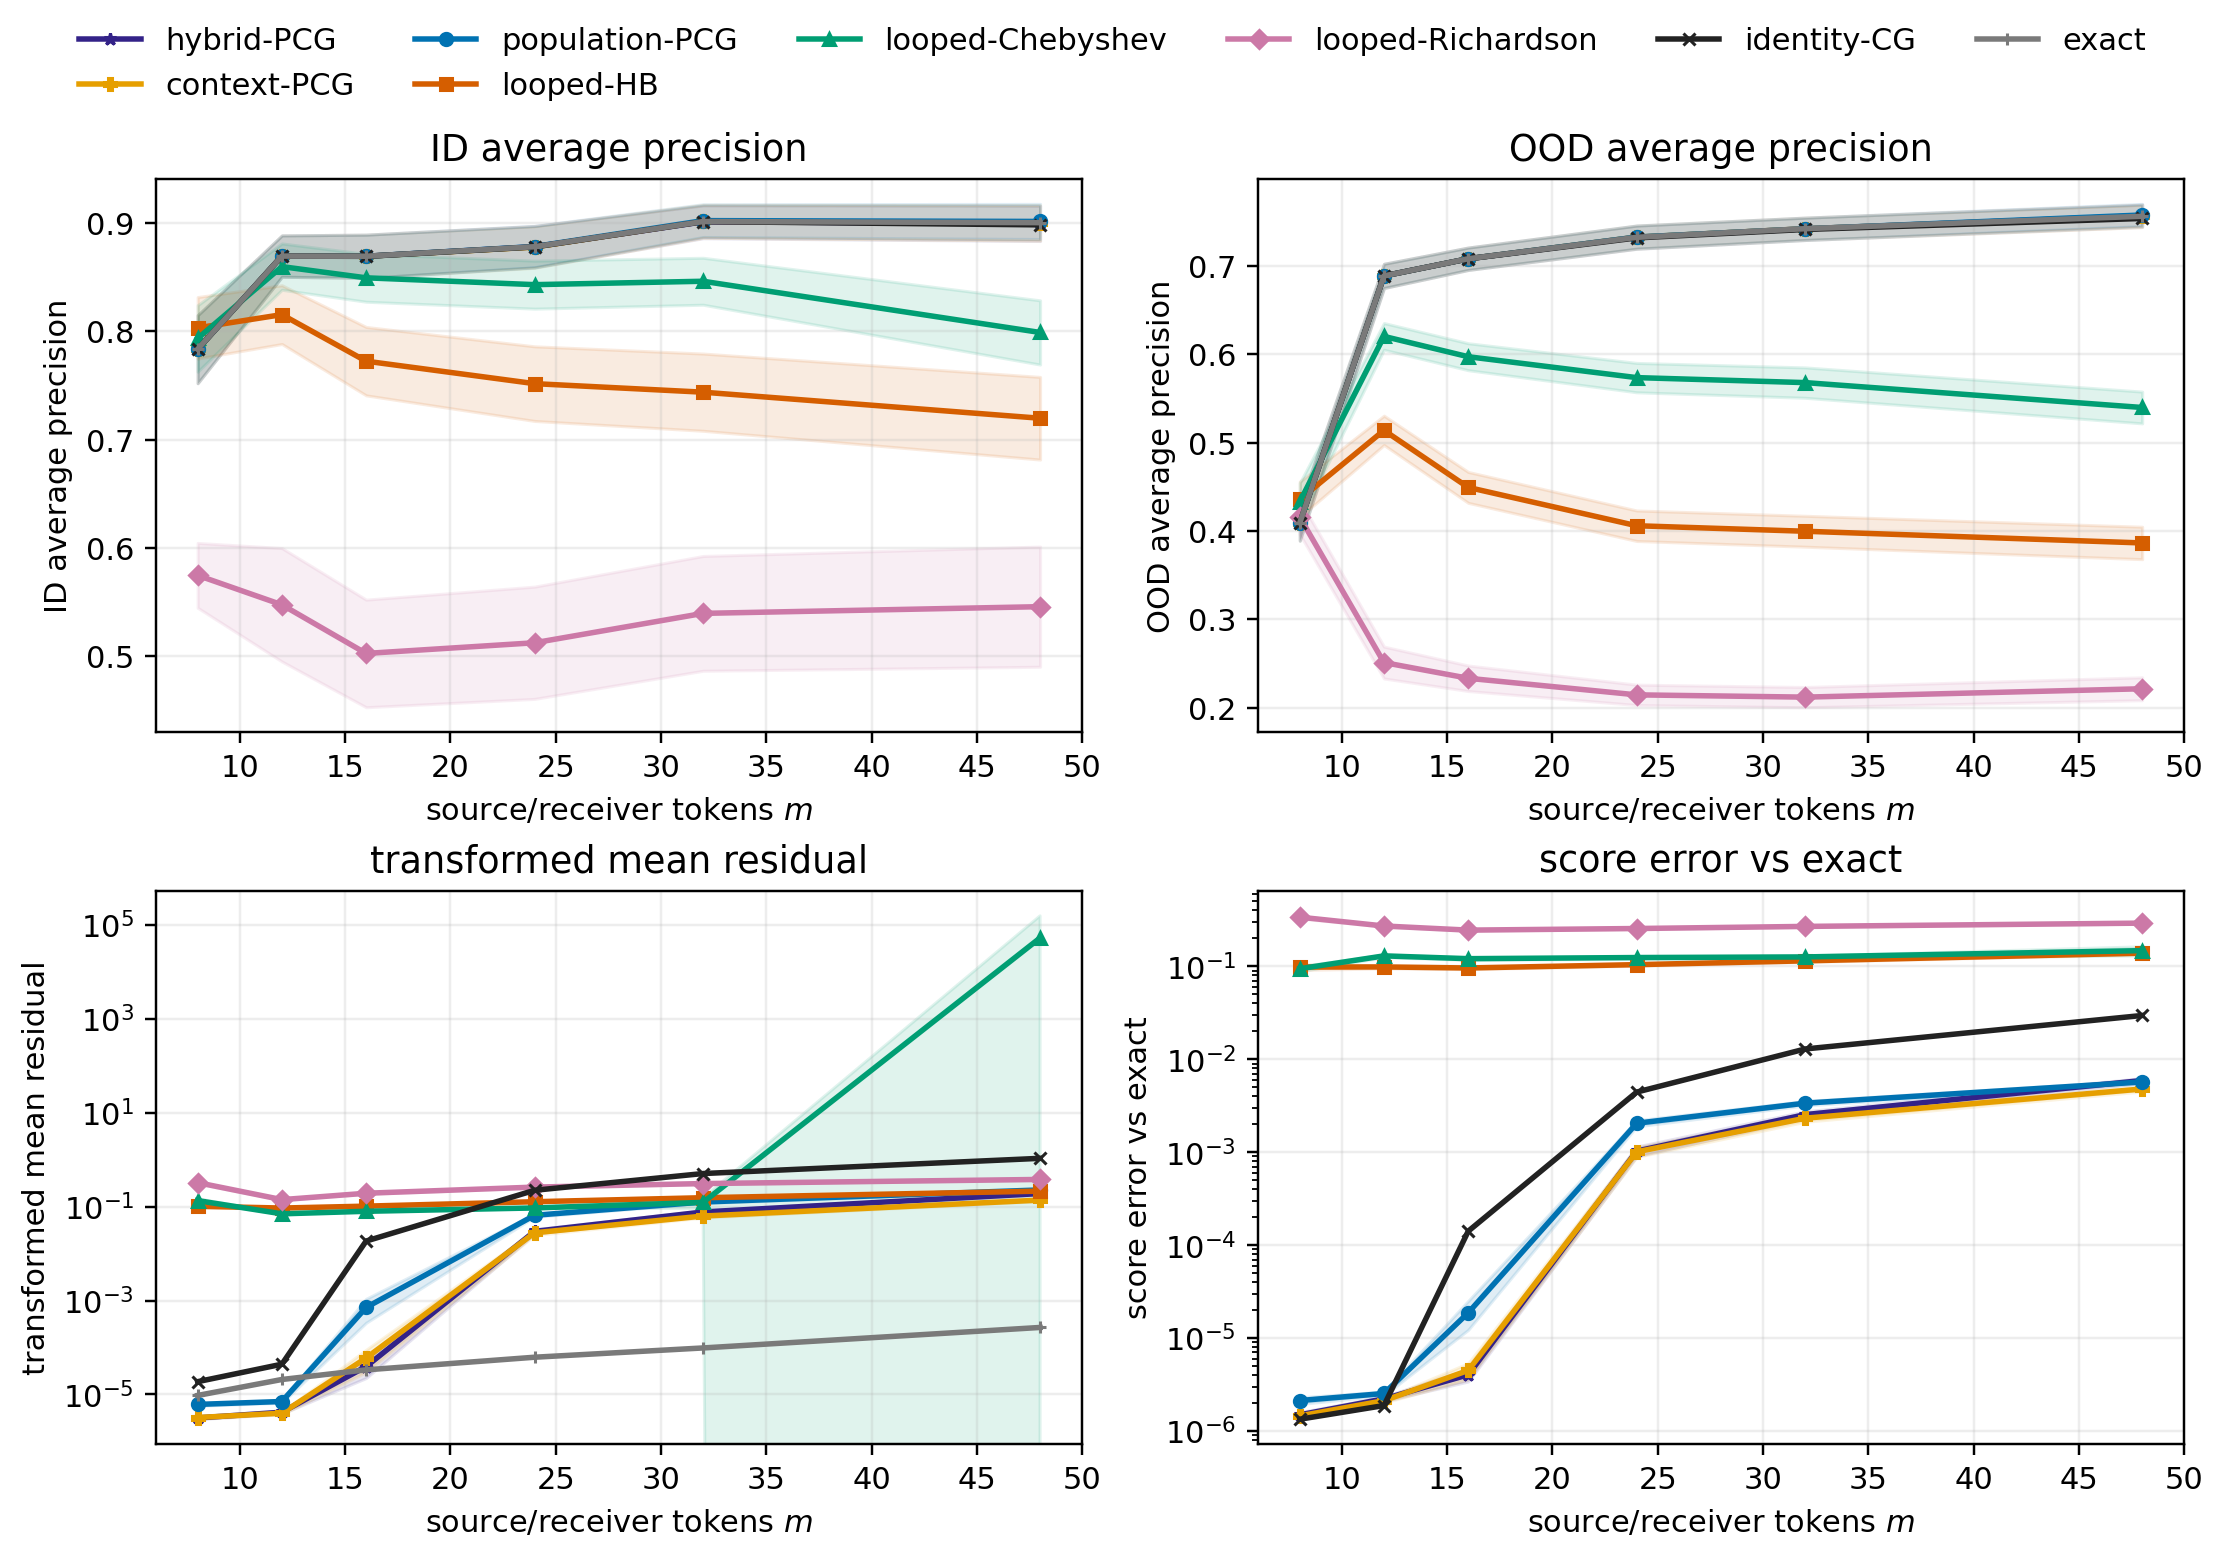
\includegraphics[width=0.98\linewidth]{scaling_context.png}
\caption{Context-length scaling.  Context $m=8$ and $m=48$ are outside the
training context set.}
\end{figure}

\begin{figure}[t]
\centering
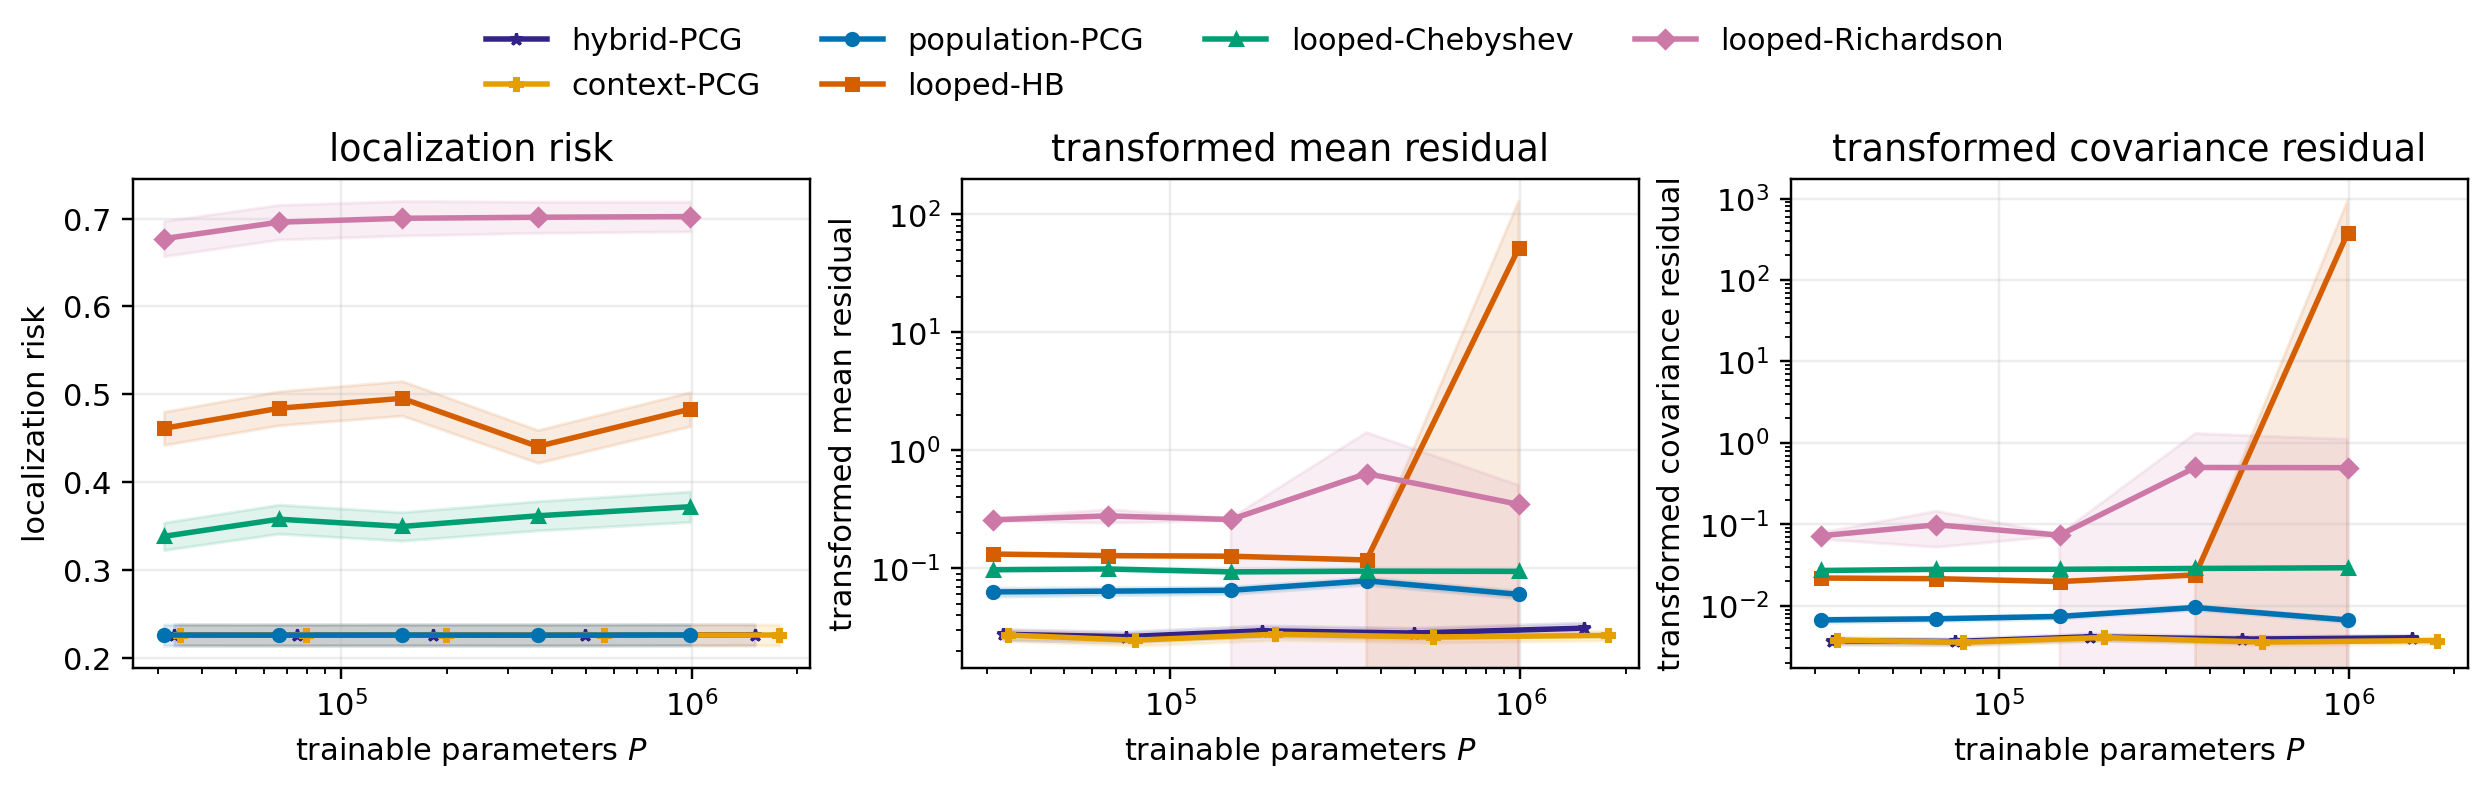
\includegraphics[width=0.98\linewidth]{scaling_network.png}
\caption{Network-size scaling at the largest completed dataset size.}
\end{figure}

\begin{figure}[t]
\centering
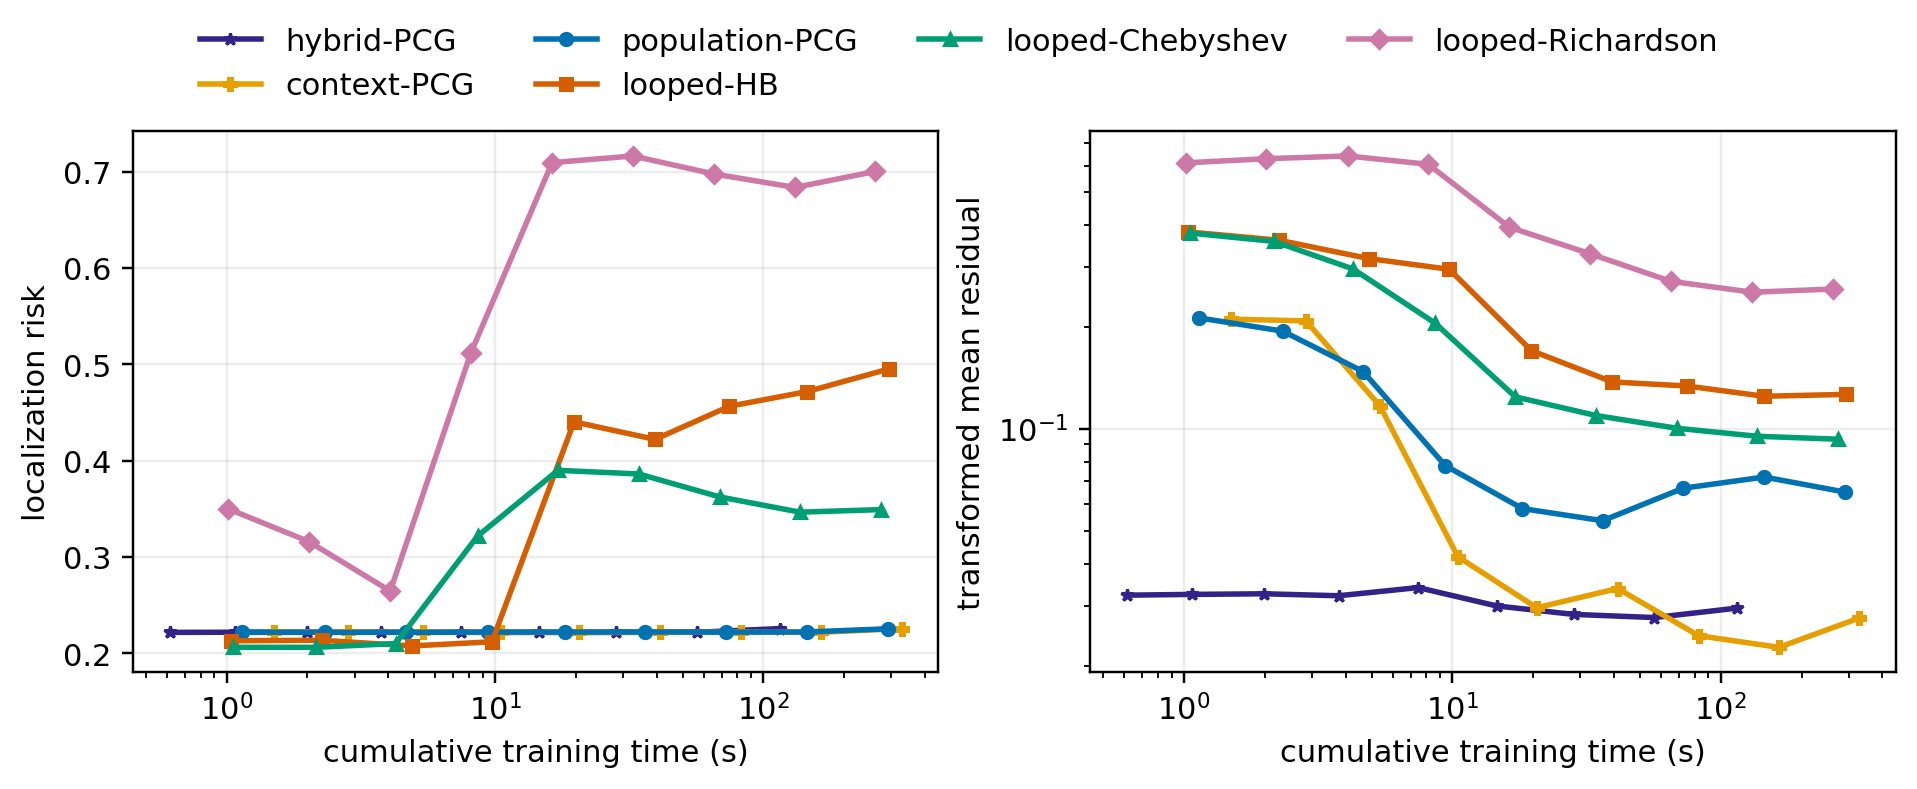
\includegraphics[width=0.9\linewidth]{scaling_time.png}
\caption{Wall-clock learning curves.  Time includes physical task generation,
forward/backward propagation and optimization, but excludes held-out audits.
Curves use the median over seeds because the accelerator is shared.}
\end{figure}

\begin{figure}[t]
\centering
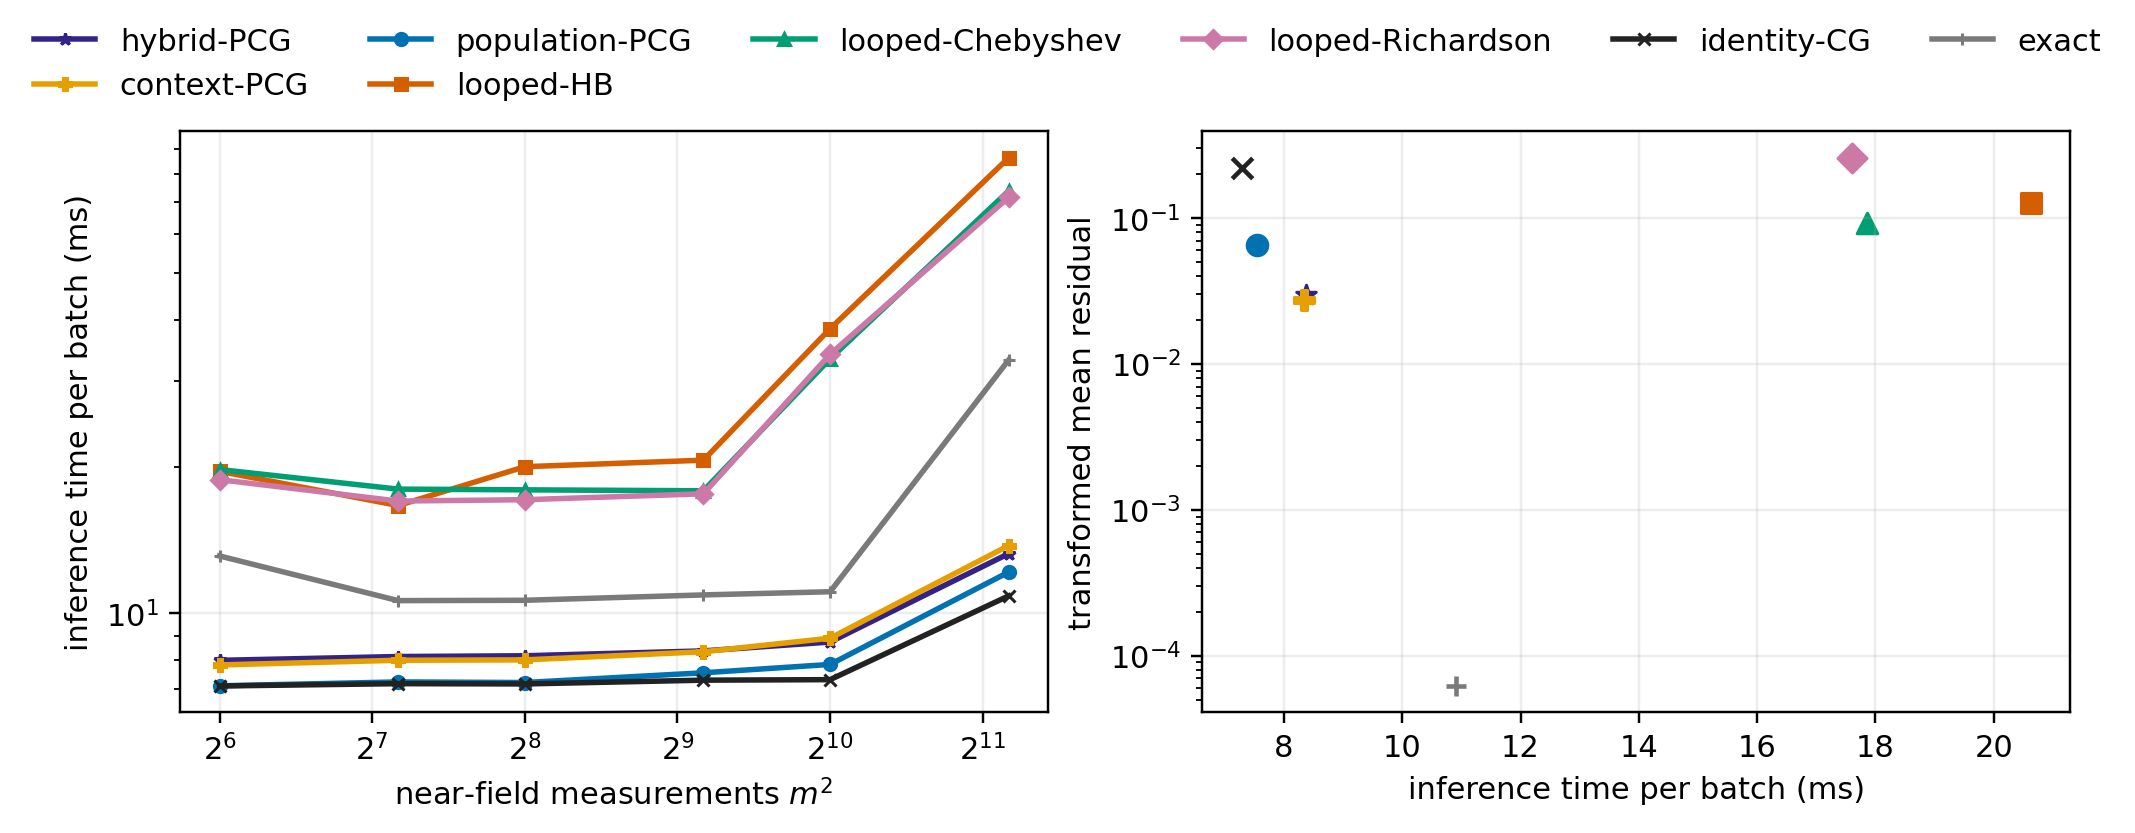
\includegraphics[width=0.95\linewidth]{scaling_runtime.png}
\caption{Inference scaling with $m^2$ complex measurements and the
residual--time Pareto comparison at $m=24$.}
\end{figure}


\begin{figure}[t]
\centering
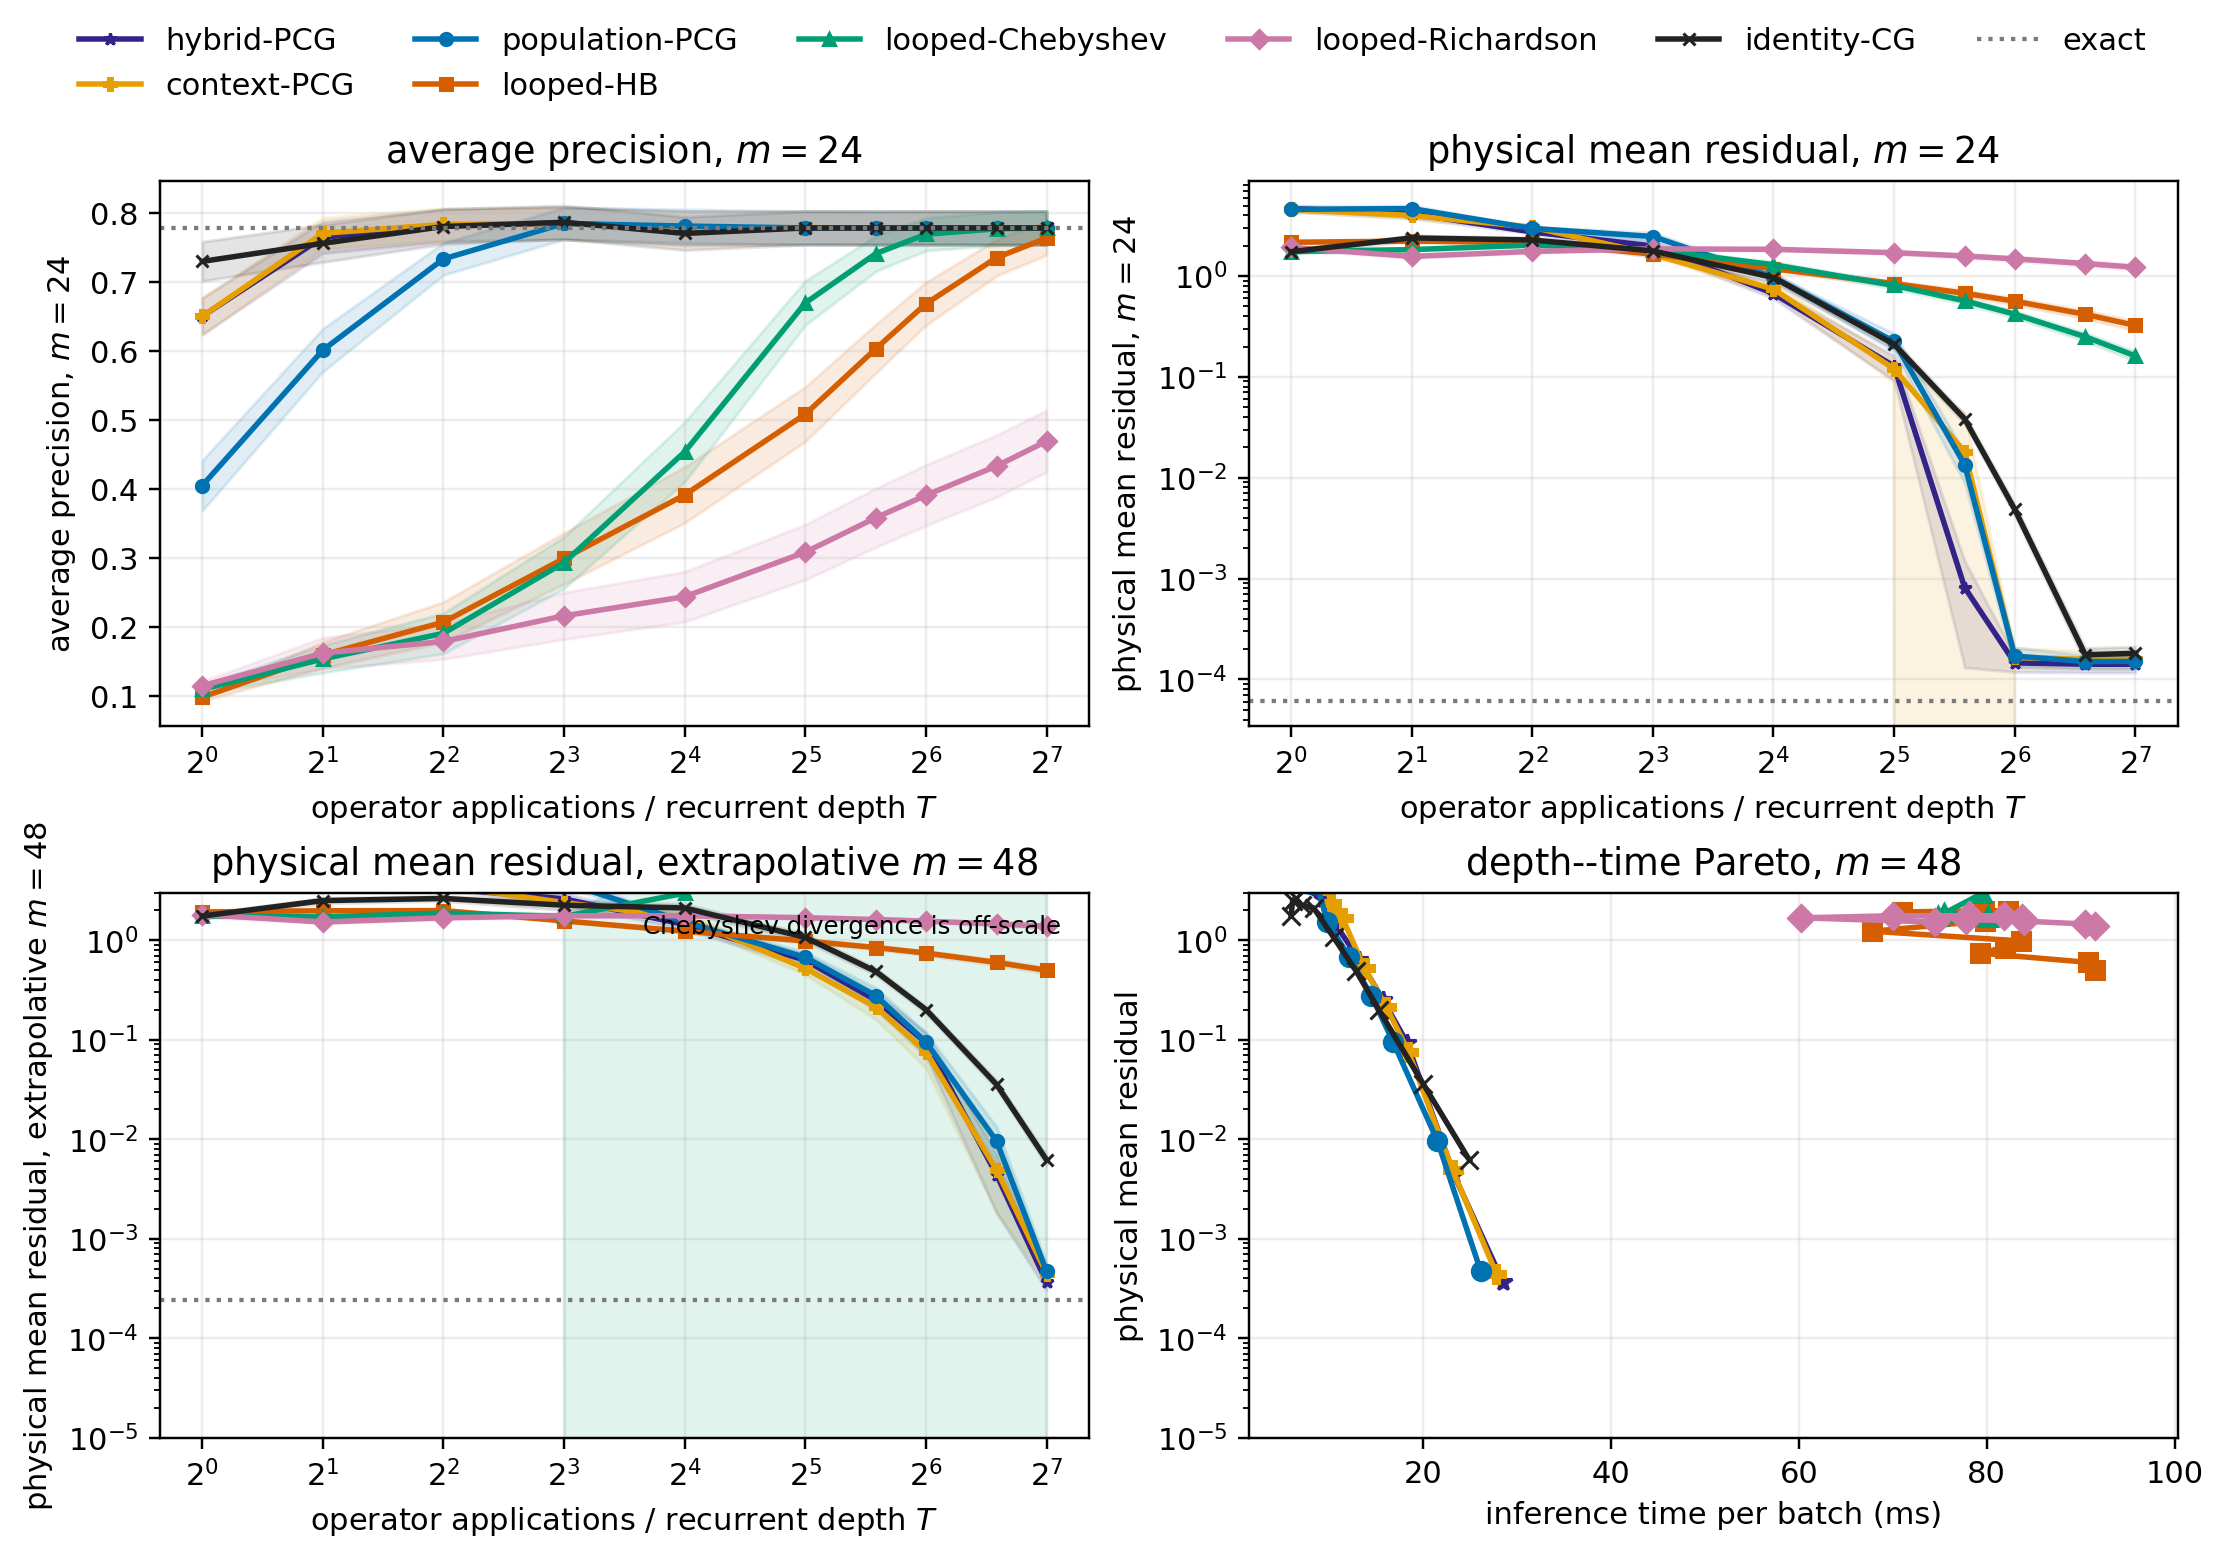
\includegraphics[width=0.98\linewidth]{scaling_depth.png}
\caption{Post-training depth scaling on shared held-out tasks.  Varying $T$
changes only the number of operator applications; parameters and acquisition
data are fixed.  The lower-right panel reports the realized depth--time Pareto
curve rather than assuming ideal linear timing.}
\label{fig:depth}
\end{figure}



\begin{figure}[t]
\centering
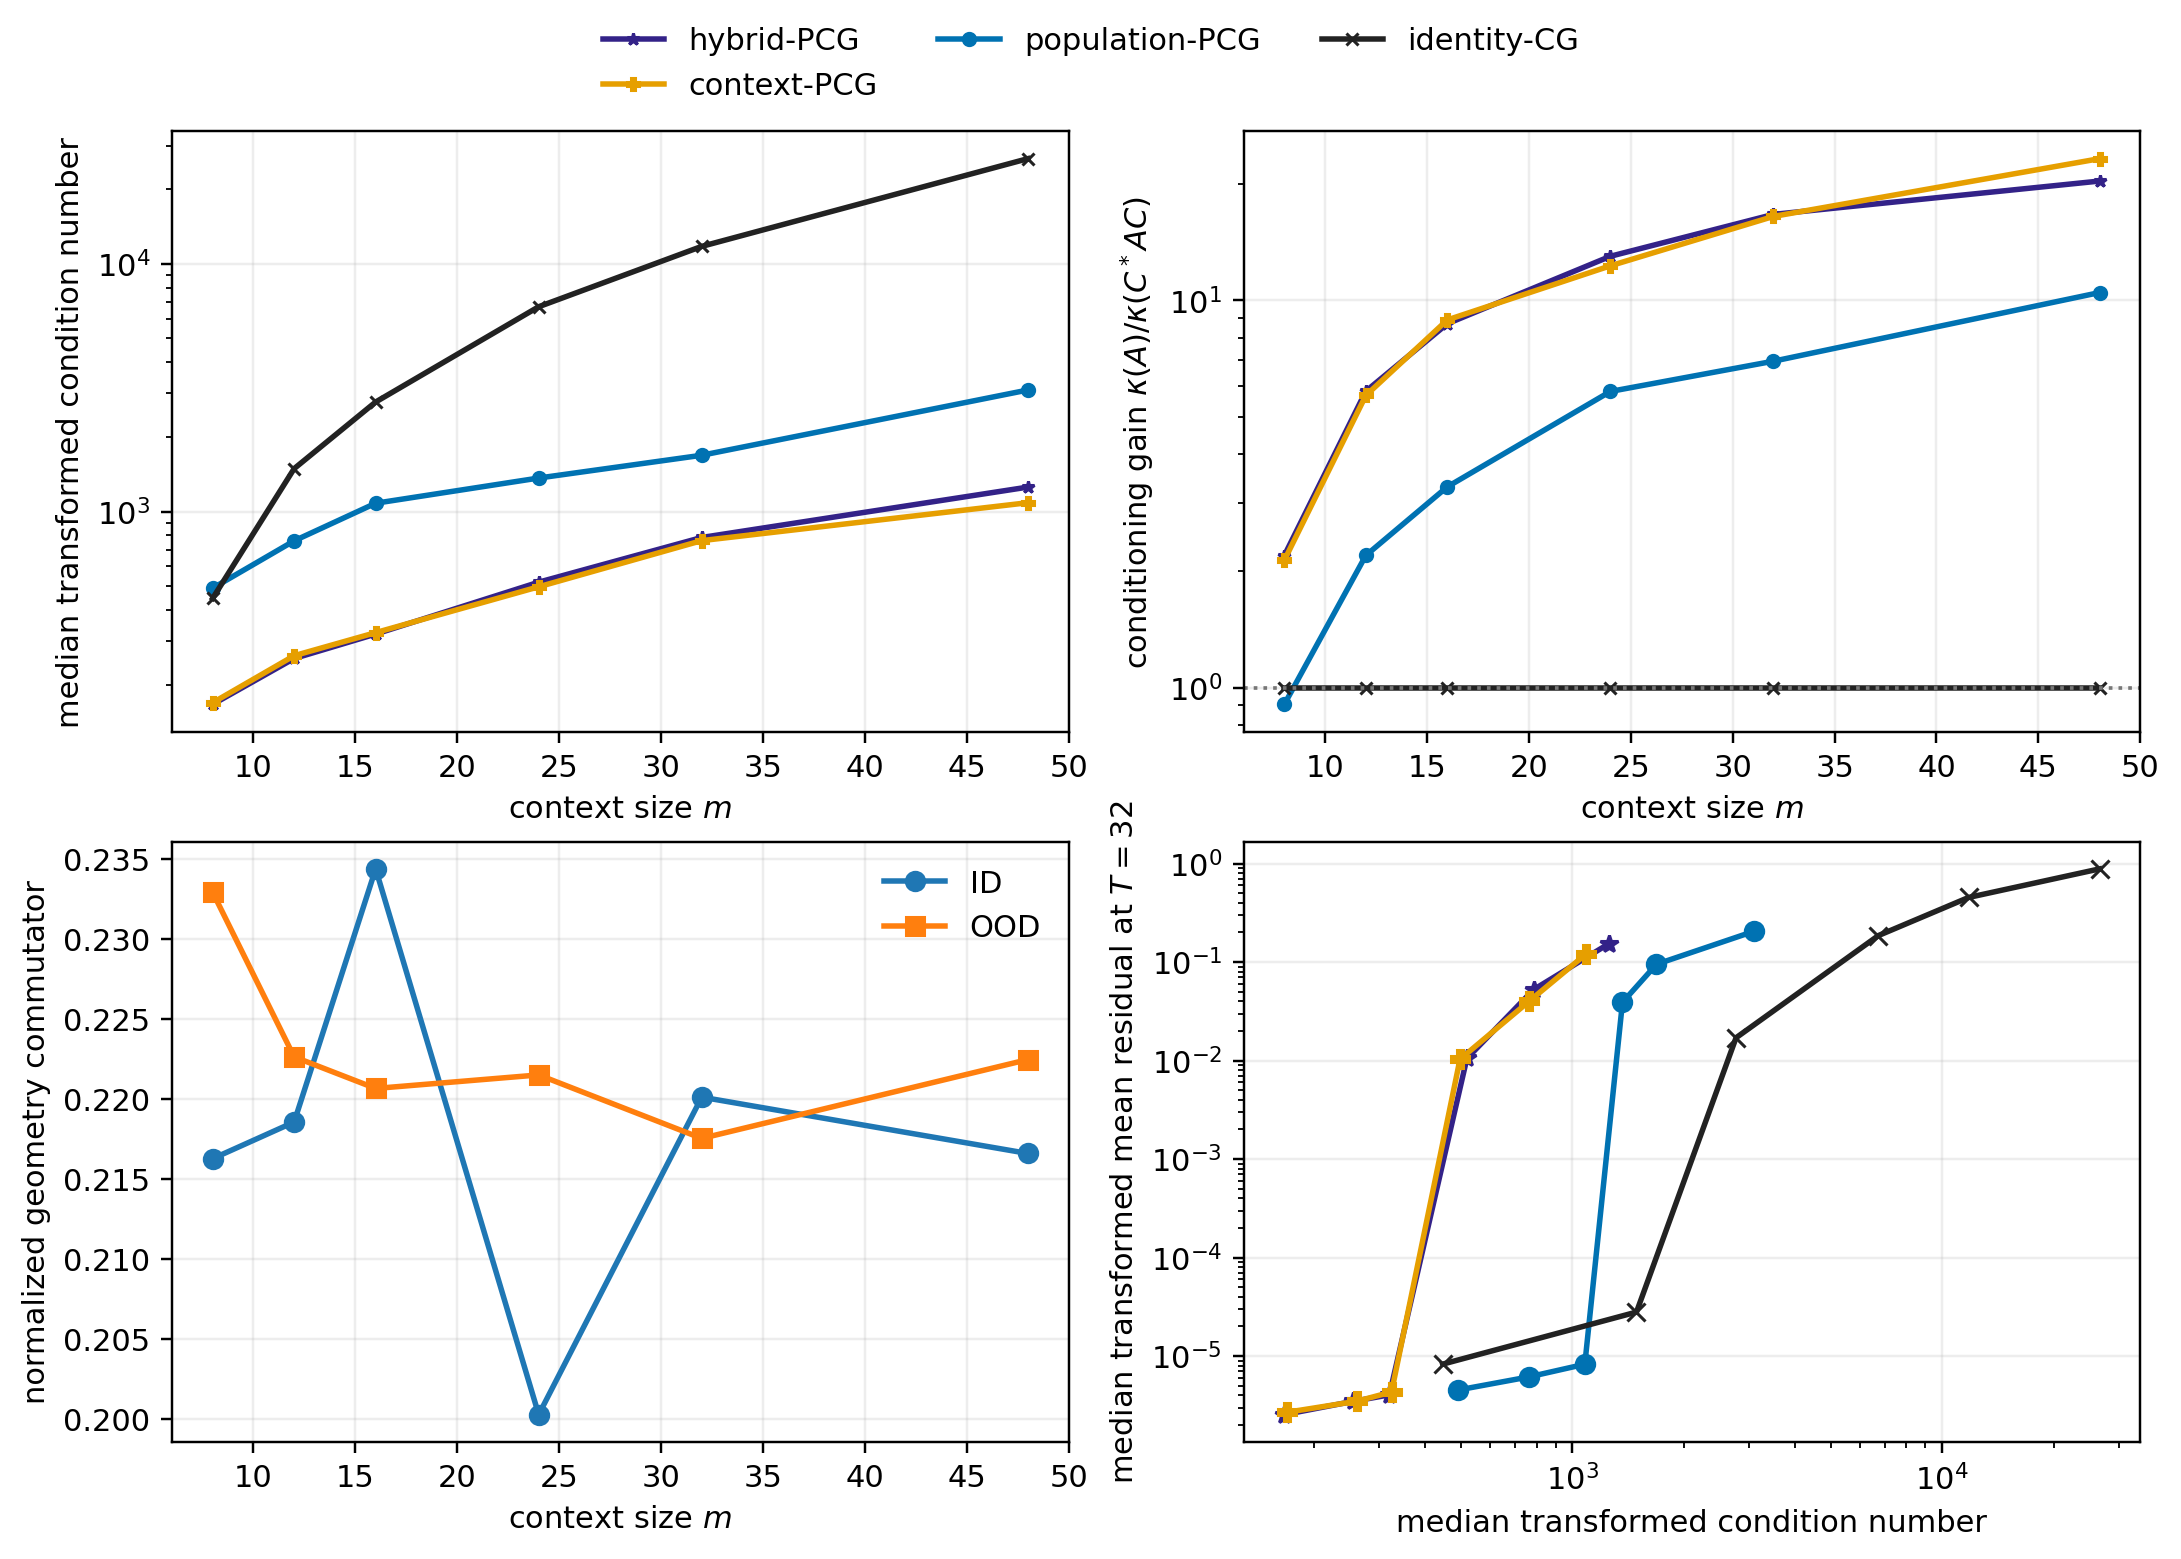
\includegraphics[width=0.98\linewidth]{scaling_conditioning.png}
\caption{Spectral conditioning audit.  The normalized commutator tests the
alignment of the fixed angular-kernel basis with the obstacle-dependent
near-field Hessian; values away from zero expose a fixed-basis bottleneck.}
\label{fig:conditioning}
\end{figure}



\begin{figure}[t]
\centering
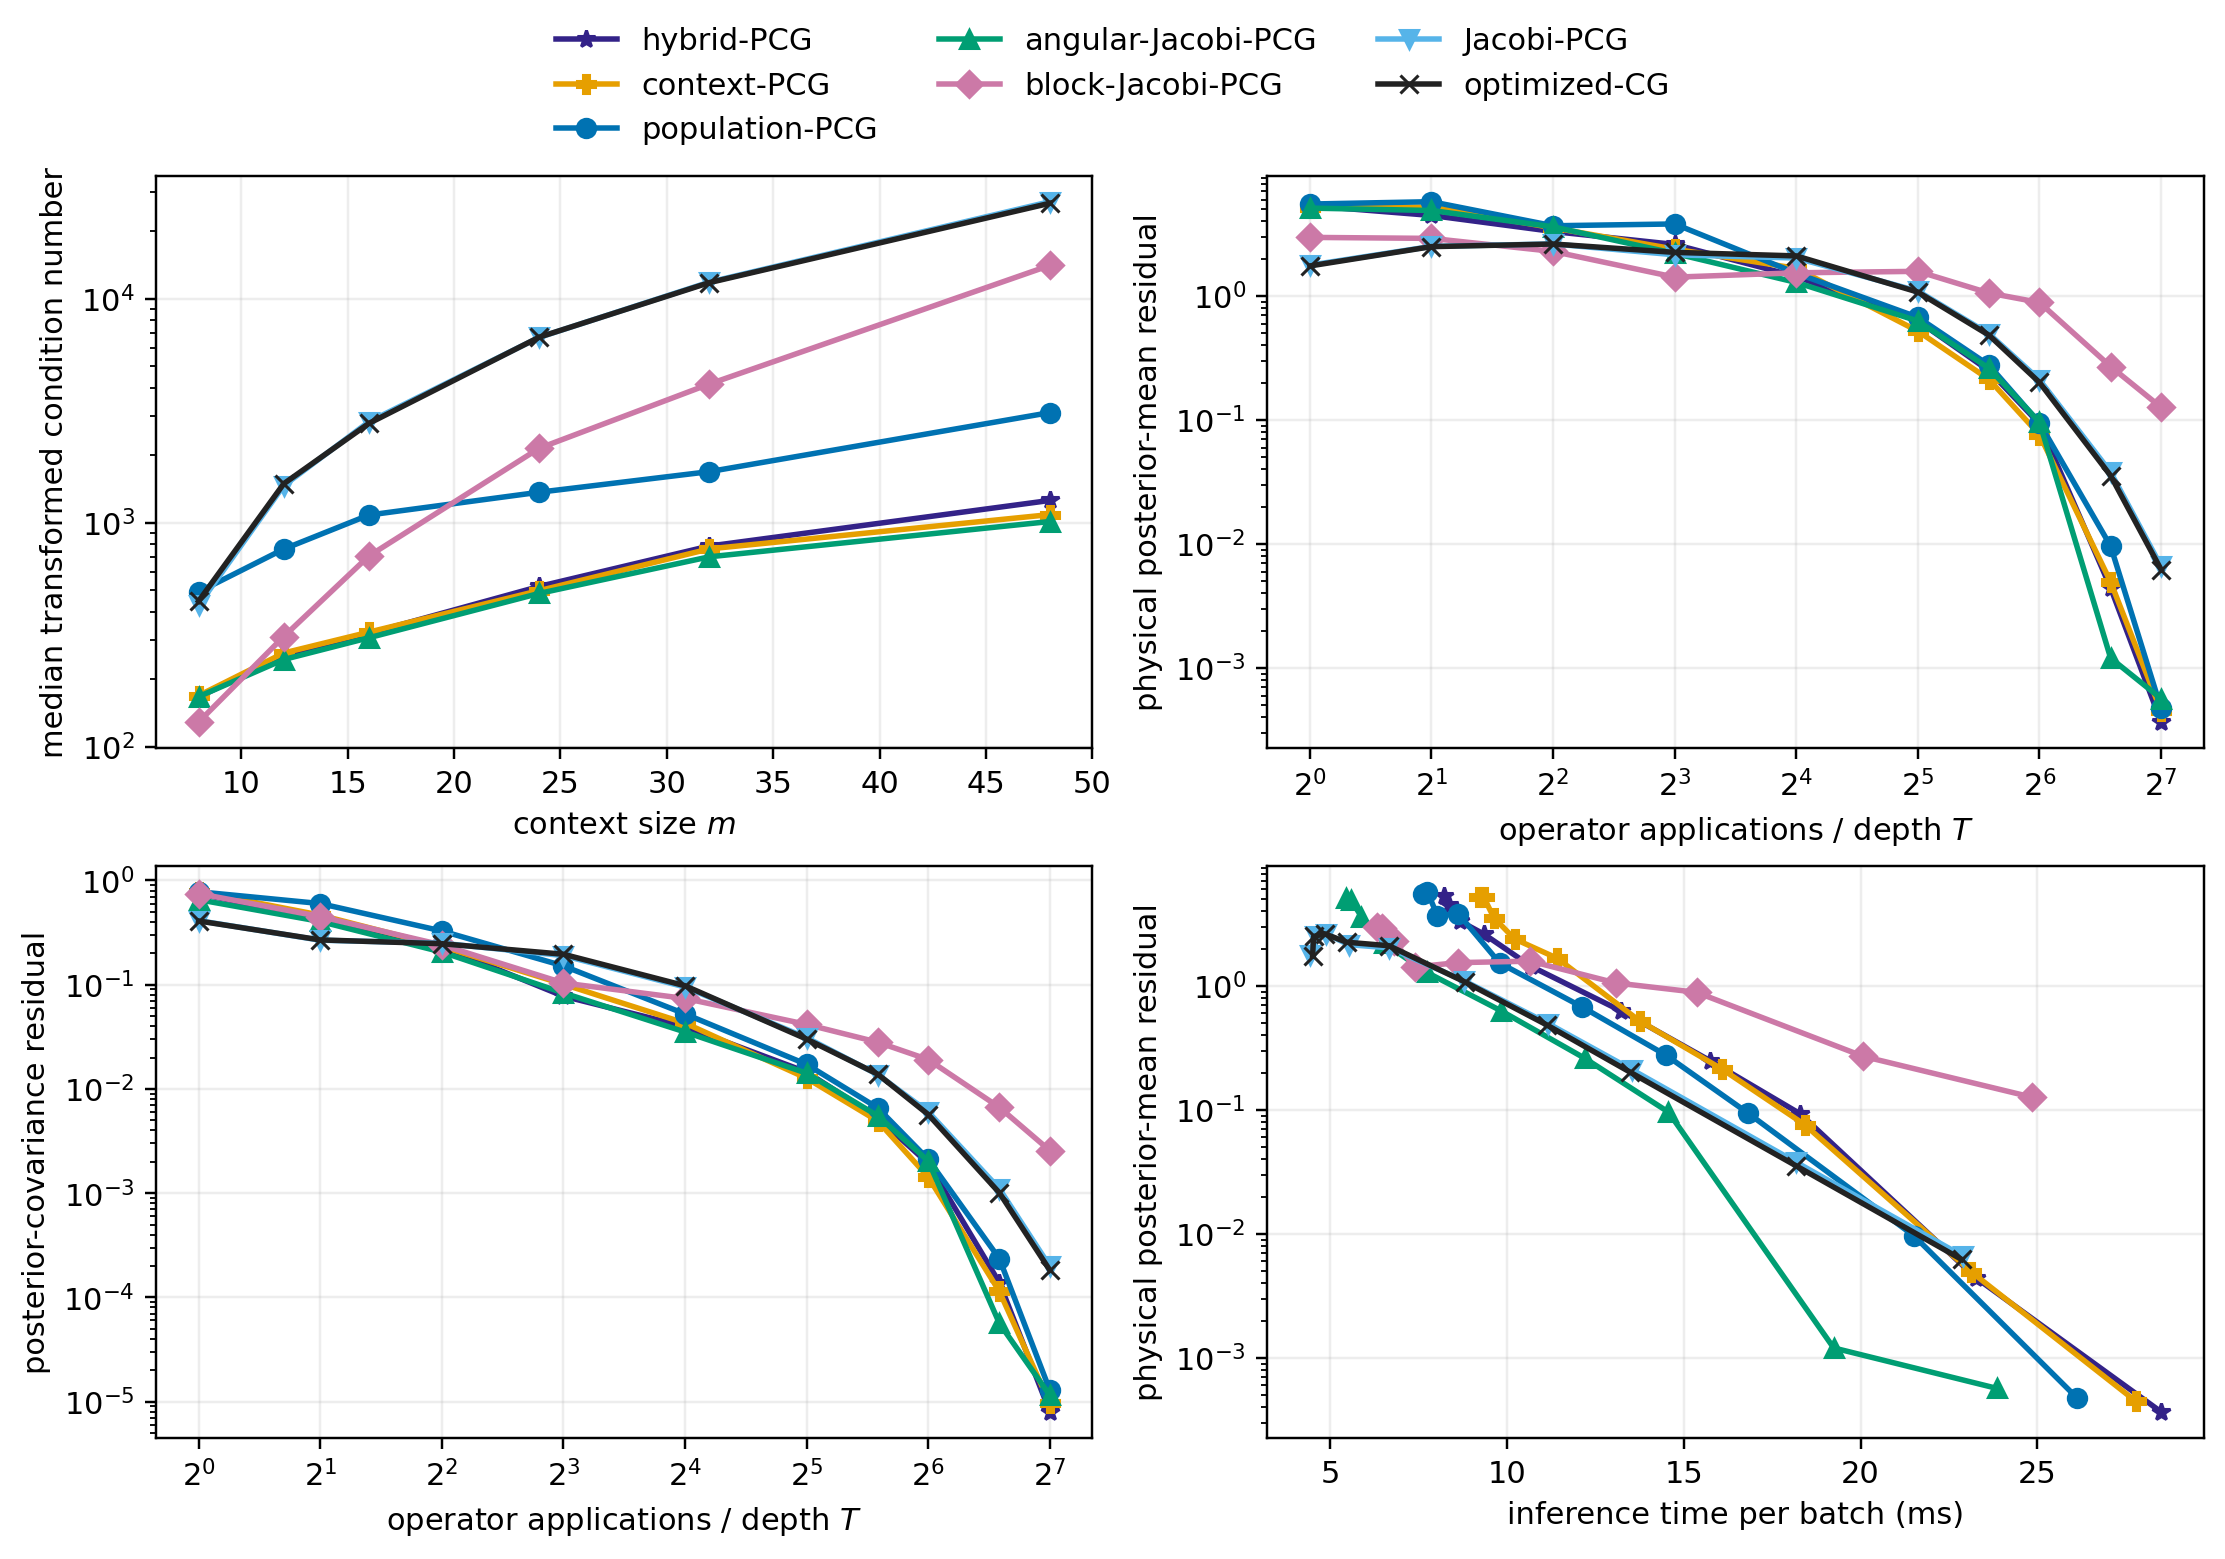
\includegraphics[width=0.98\linewidth]{scaling_classical_preconditioners.png}
\caption{Training-free PCG controls at matched depth.  Jacobi uses the physical
diagonal, block-Jacobi uses contiguous angular blocks of size four, and
angular-Jacobi uses the diagonal of the current Hessian in the fixed GP
angular basis.}
\label{fig:classical-pcg}
\end{figure}



\begin{figure}[t]
\centering
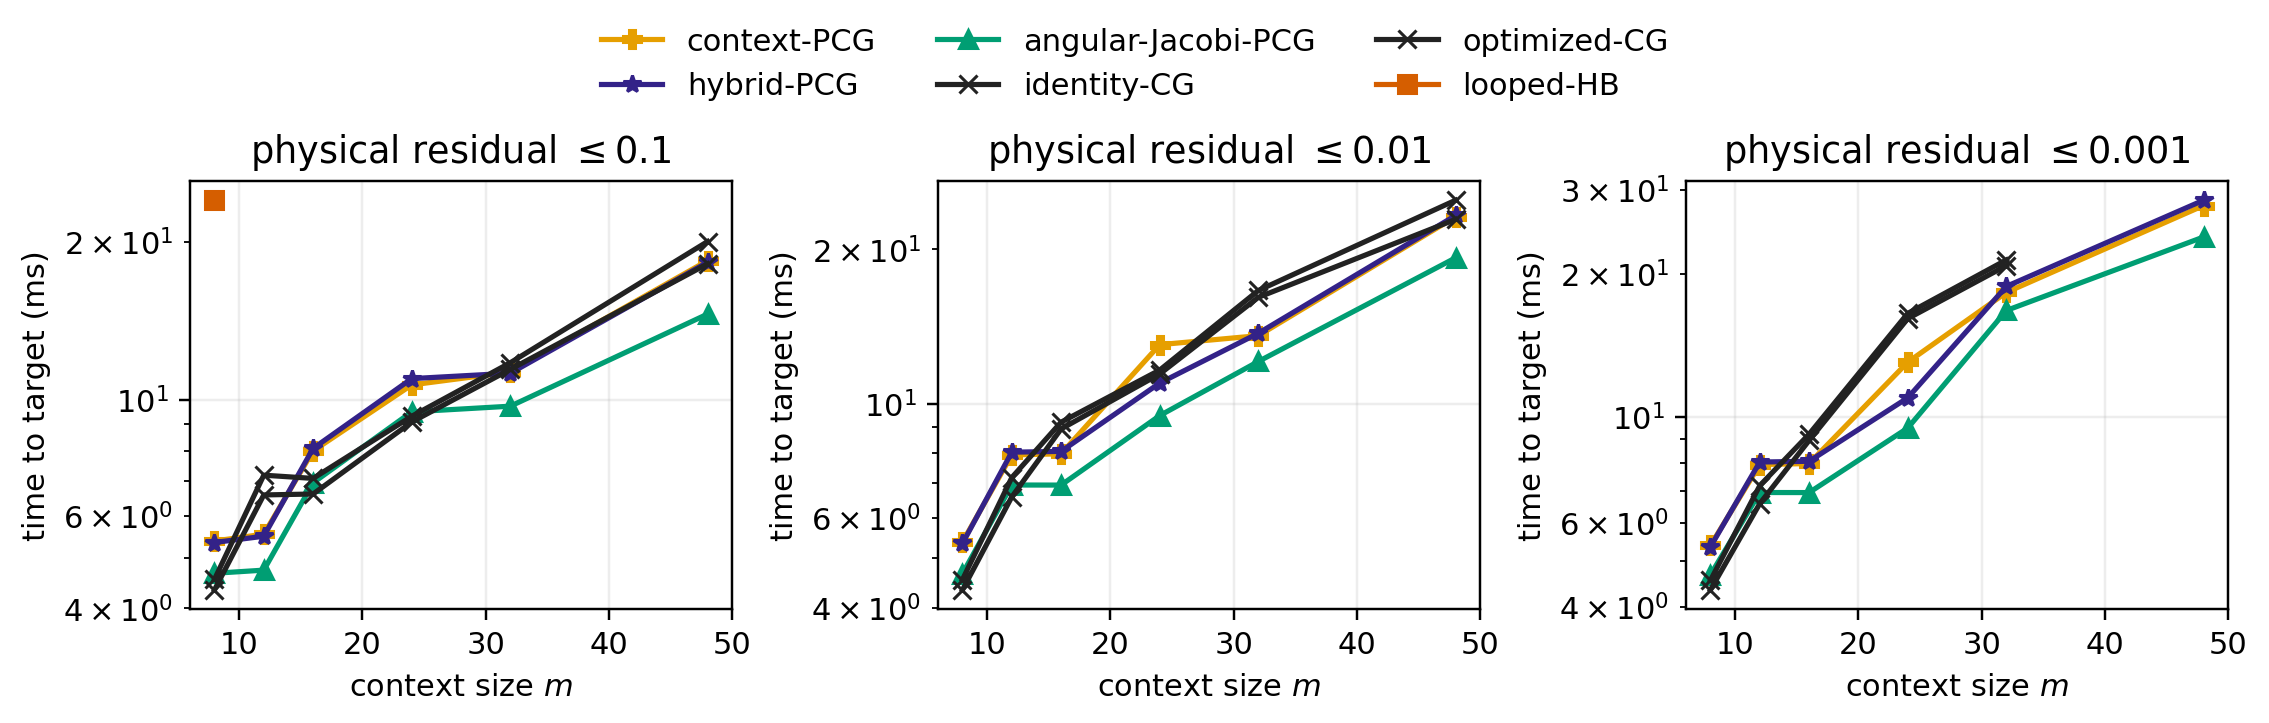
\includegraphics[width=0.98\linewidth]{scaling_tolerance_frontier.png}
\caption{Measured time to residual targets on the audited depth grid.  A curve
is absent where a method does not reach the target by $T=128$.  Equal-depth and
time-to-tolerance comparisons need not rank methods identically.}
\label{fig:tolerance-frontier}
\end{figure}



\begin{figure}[p]
\centering
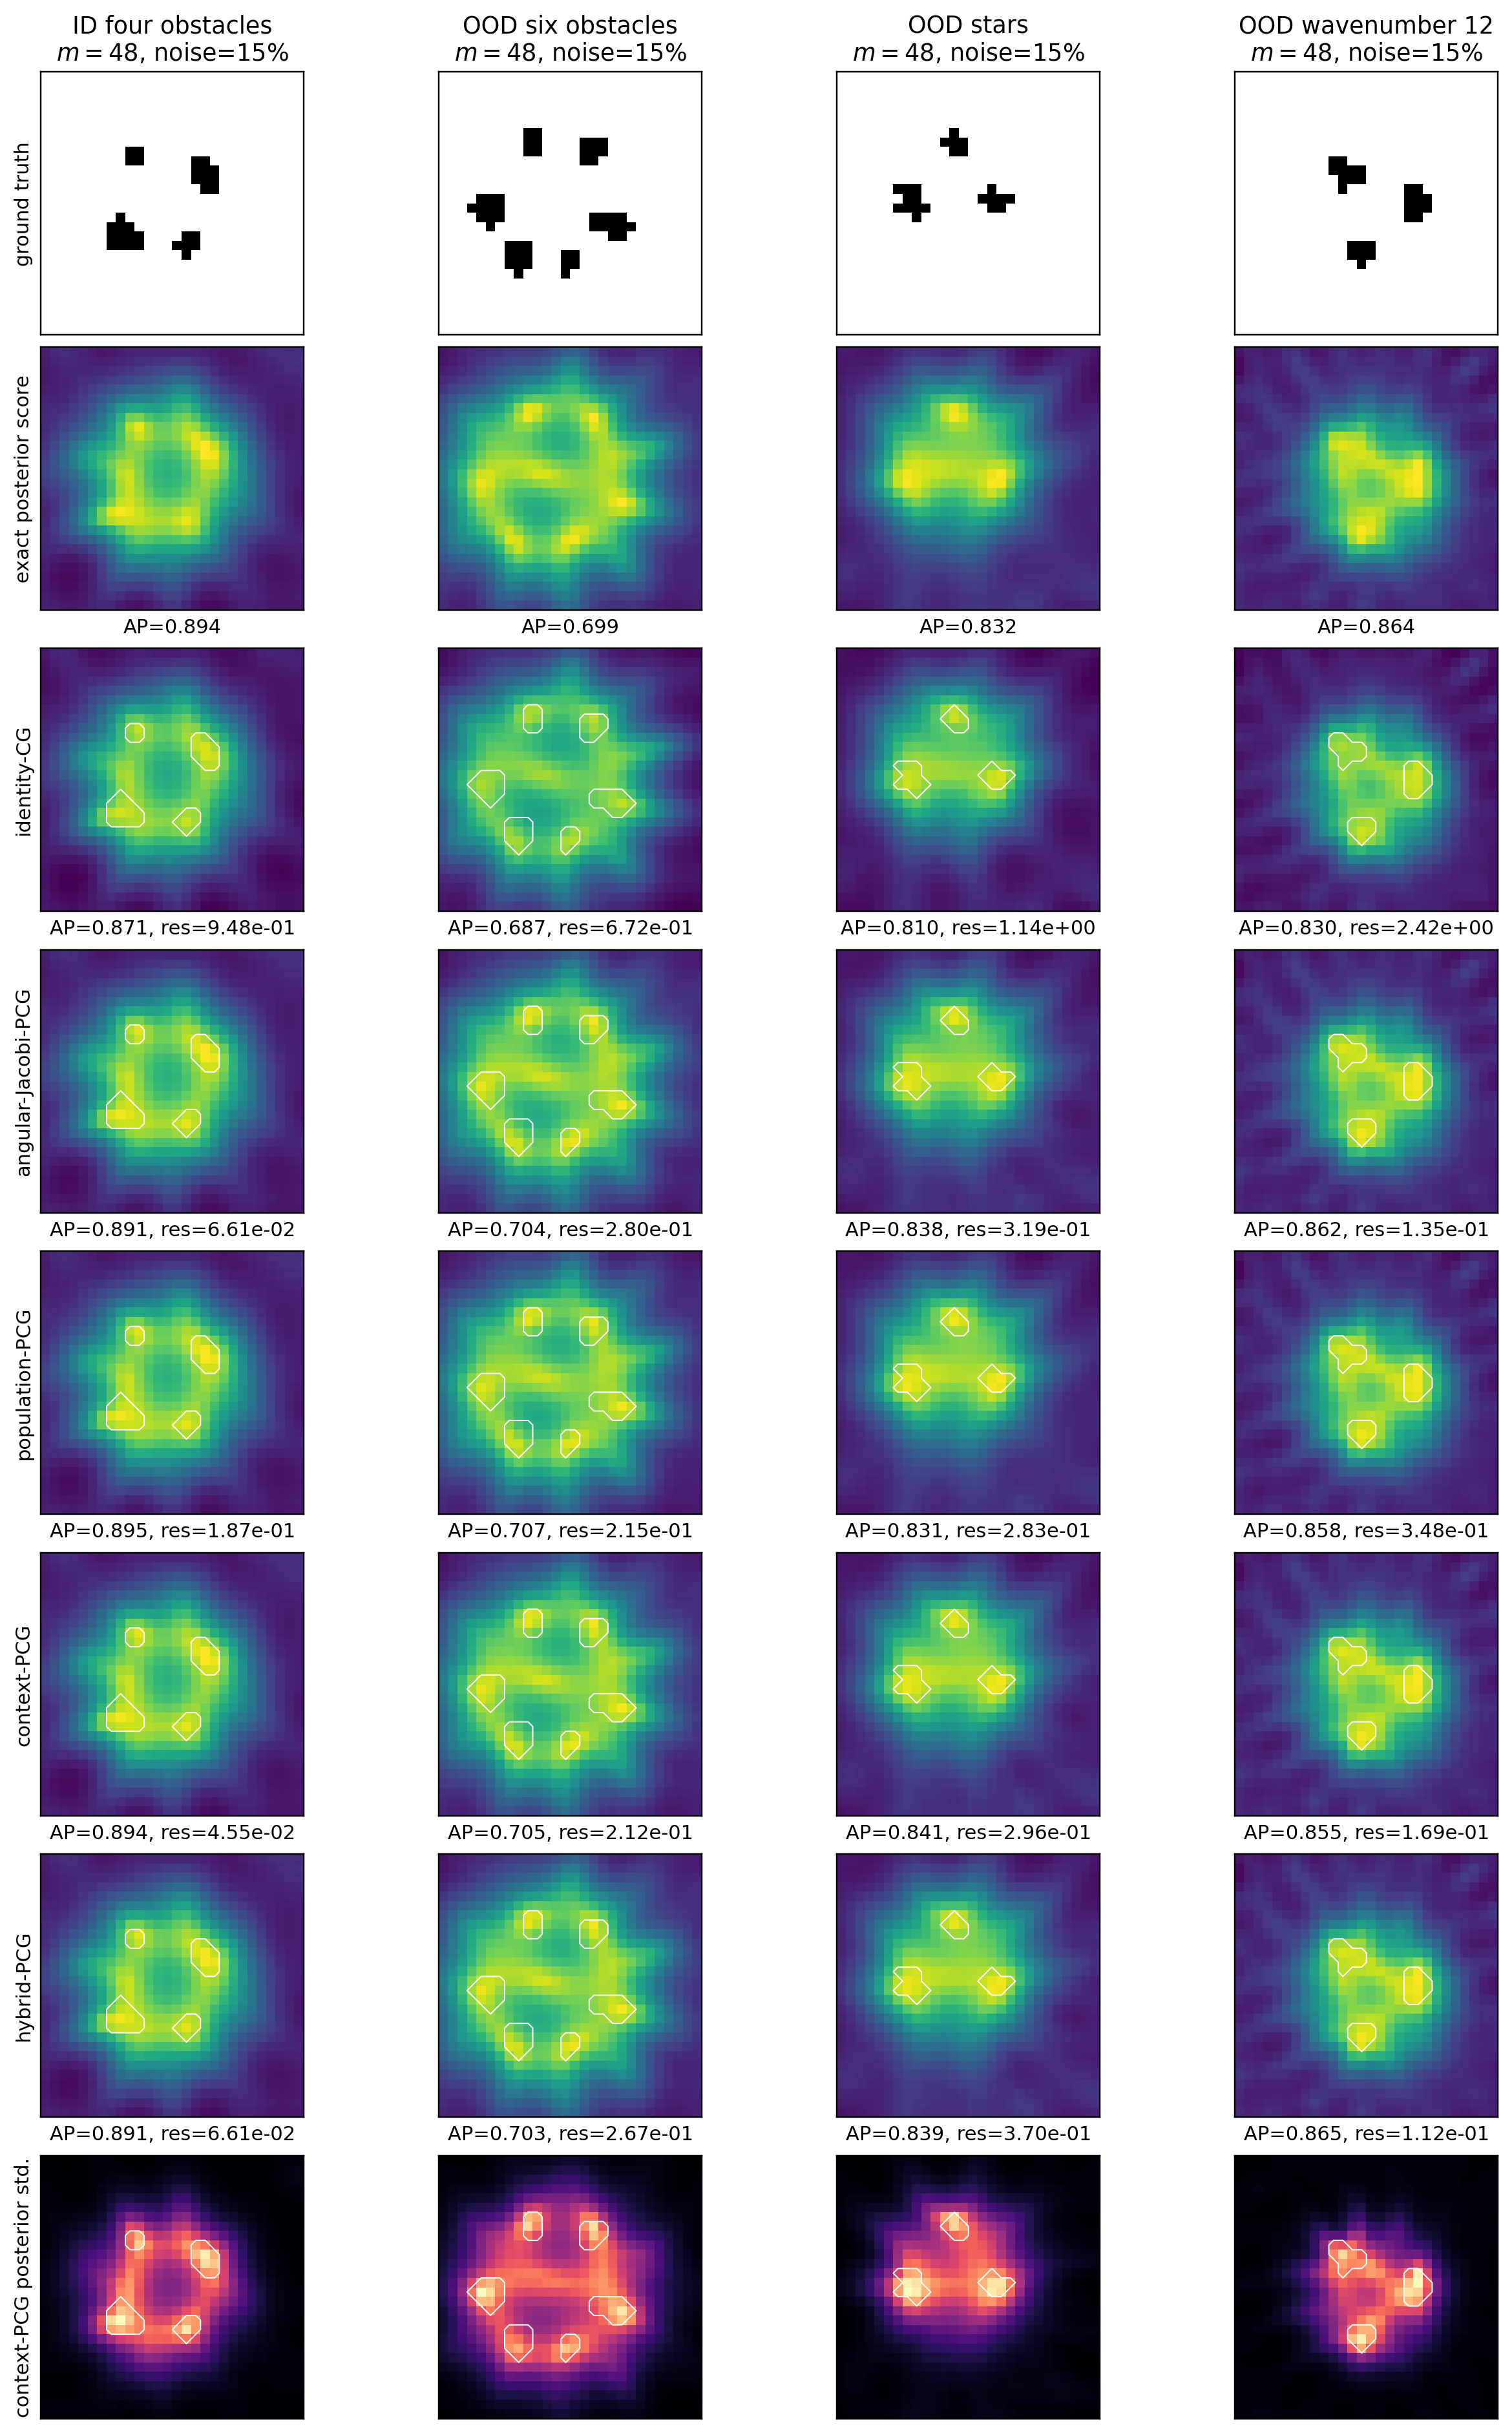
\includegraphics[width=0.94\linewidth,height=0.84\textheight,keepaspectratio]{scaling_reconstructions.png}
\caption{Pre-specified task zero at extrapolative context $m=48$; no example
was selected by performance.  White contours show the true obstacles.  The
rows compare CG, analytic angular-Jacobi PCG, the learned factors, and the
analytic--learned hybrid.  The last row displays context-PCG posterior standard
deviation rather than a reconstruction score.}
\label{fig:reconstructions}
\end{figure}


\FloatBarrier
\section{Interpretation and limitations}
Six claims are deliberately separated.  First, CG is a strong task-adaptive
baseline because its coefficients already depend on the current Krylov space.
Second, population-PCG tests whether geometry-distribution conditioning adds
value when no obstacle-specific preconditioner is known.  Third, context-PCG
tests prompt-dependent modal gains while keeping the angular-kernel basis
fixed.  Fourth, hybrid-PCG tests whether a bounded learned correction adds to
the analytic GP-basis diagonal.  Fifth, looped HB tests amortized fixed-depth
iteration, not a universally superior replacement for CG.  Sixth,
angular-Jacobi-PCG tests whether the same task signal can be extracted
analytically without training.
A fully equivariant task-specific
preconditioner would map current moment or Ritz information into an SPD
operator $C_D(A_D)\approx A_D^{-1/2}$.  Neither modal model can rotate all
obstacle-dependent eigendirections; a block-Lanczos or polynomial-in-$A_D$
extension is required when the commutator audit is large.
The joint-shift audit also shows that nearly equal condition numbers can have
different finite-depth residuals.  A next loop should therefore encode the
right-hand-side-weighted spectral measure through moments
$B^*A_D^jB$, not only extremal eigenvalues or scalar condition number; exact
outer Krylov coefficients can then preserve the CG guarantee.

The held-out bound certifies the stated simulator distribution only.  The
forward data are generated by MFS, not laboratory measurements, and context
extrapolation does not imply robustness to arbitrary receiver geometries.
Physical resolution remains controlled by aperture, frequency and sensor
count.  These qualifications prevent a small numerical loss from being
misreported as solved inverse scattering.

\section{Reproducibility}
All task-level records, cumulative training times, checkpoints, runtime
measurements, scenario definitions, fitted parameters and bound values are
stored beside this PDF.  The experiment uses three fixed seeds and preserves
the exact same held-out tasks across methods, widths and dataset checkpoints.

\begin{thebibliography}{9}
\bibitem{bordelon2025} B. Bordelon, M. I. Letey, and C. Pehlevan.
Theory of scaling laws for in-context regression: depth, width, context and
time. \emph{arXiv:2510.01098}, 2025.
\bibitem{kang2026} G. Kang, C. J. Lee, and X. Cheng.
Transformers can learn posterior predictive distributions in-context.
\emph{arXiv:2605.26713}, 2026.
\bibitem{garnier2022} J. Garnier, H. Haddar, and H. Montanelli.
The linear sampling method for random sources. \emph{arXiv:2210.15560}, 2022.
\bibitem{garnier2024} J. Garnier, H. Haddar, and H. Montanelli.
The linear sampling method for data generated by small random scatterers.
\emph{arXiv:2403.19482}, 2024.
\bibitem{polyak1964} B. T. Polyak. Some methods of speeding up the convergence
of iteration methods. \emph{USSR Computational Mathematics and Mathematical
Physics}, 1964.
\bibitem{saad2003} Y. Saad. \emph{Iterative Methods for Sparse Linear
Systems}, second edition, SIAM, 2003.
\end{thebibliography}
\end{document}
